\documentclass[journal,twoside,web]{ieeecolor}
\usepackage{jsen}
\usepackage{cite}
\usepackage{amsmath,amssymb,amsfonts}
\usepackage{algorithmic}
\usepackage{graphicx}
\usepackage{textcomp}
\usepackage{wrapfig}
\usepackage{url}
\usepackage{tabularx}
\usepackage{array}
\usepackage{afterpage}
\usepackage{booktabs}
\usepackage{makecell}



\def\BibTeX{{\rm B\kern-.05em{\sc i\kern-.025em b}\kern-.08em
    T\kern-.1667em\lower.7ex\hbox{E}\kern-.125emX}}
\markboth{\journalname, VOL. XX, NO. XX, XXXX 2026}
{Author \MakeLowercase{\textit{et al.}}: Measurement-Law-Constrained Physics-Informed Inverse Learning for Single-Sensor FBG Thermo-Mechanical Estimation}
\definecolor{abstractbg}{rgb}{0.89804,0.94510,0.83137}
\setlength{\fboxrule}{0pt}
\setlength{\fboxsep}{0pt}

\begin{document}
\title{Single-Fiber-Bragg-Grating Thermo-Mechanical Estimation as a Measurement-Law-Constrained Inverse-Learning Problem: A Physics-Informed Neural Network Study}
\author{Anvitha Anant Rao, Srivanth Srinivasan, and Somesh Nandi, \IEEEmembership{Member, IEEE}
\thanks{This paragraph of the first footnote will contain the date on
which you submitted your paper for review. It will also contain support
information, including sponsor and financial support acknowledgment.}
\thanks{Anvitha Anant Rao is with the Department of Artificial Intelligence and Machine Learning, R. V. College of Engineering, Bengaluru, India (e-mail: anvithaanantr.ai22@rvce.edu.in). }
\thanks{Srivanth Srinivasan is with the Department of Artificial Intelligence and Machine Learning, R. V. College of Engineering, Bengaluru, India (e-mail: srivanths.ai22@rvce.edu.in).}
\thanks{Somesh Nandi is with the Department of Artificial Intelligence and Machine Learning, R. V. College of Engineering, Bengaluru, India (e-mail: someshnandi@rvce.edu.in).}}

\IEEEtitleabstractindextext{%
\fcolorbox{abstractbg}{abstractbg}{%
\begin{minipage}{\textwidth}%
\hspace{0.6em}%
\begin{minipage}{\dimexpr\textwidth-1.2em}
\color{black}
\vspace{0.3em}
\setlength{\baselineskip}{1.1\baselineskip}

\setlength{\intextsep}{1em}
\setlength{\columnsep}{2.2em}

\begin{wrapfigure}[14]{r}{3.1in}
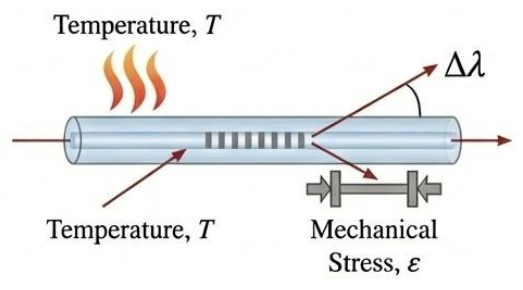
\includegraphics[width=2.9in]{abstract.png}
\end{wrapfigure}

\begin{abstract}
\indent
A single Fiber Bragg Grating (FBG) sensor reports one scalar quantity, the
Bragg wavelength shift, yet its response depends on two independent physical
causes, axial strain and temperature. Recovering both from that single
observation is therefore a fundamentally ill-posed inverse problem: the
measurement law admits infinitely many strain-temperature pairs that
reproduce any given wavelength shift. This paper formulates single-FBG
thermo-mechanical estimation as a measurement-law-constrained, partially
supervised inverse-learning problem, and experimentally investigates whether
physics-informed regularization improves reconstruction accuracy,
robustness, data efficiency, and generalization relative to purely
data-driven alternatives. A neural network is trained using explicit
supervision from separately acquired strain-only and temperature-only
experiments, together with a physics-consistency penalty derived from the
Bragg wavelength-shift equation, so that predictions for the unlabeled
combined thermo-mechanical regime remain compatible with the sensor's
physical response. On real experimental data acquired from an FBG sensor
embedded in a stainless-steel specimen and interrogated at 5~kHz, the
proposed physics-informed neural network (PINN) achieves a wavelength
reconstruction mean absolute error (MAE) of 1.99~pm and root-mean-square
error (RMSE) of 3.05~pm ($R^2=0.99989$), outperforming linear regression,
a multilayer perceptron (MLP), support vector regression (SVR), Gaussian
process regression (GPR), and random forest baselines evaluated under
identical data, preprocessing, and splitting conditions; the corresponding
improvement over classical linear calibration in wavelength-domain
reconstruction is approximately 28$\times$ in MAE. The model degrades
gracefully under injected measurement noise up to $\sigma=10$~pm, retains
sub-2~pm accuracy when trained on only 20\% of the available data, and
remains stable under $\pm10\%$ perturbation of the sensor's sensitivity
coefficients. Because the combined thermo-mechanical regime lacks
independent ground-truth labels for strain and temperature individually, the
reported accuracy is established and interpreted at the level of wavelength
reconstruction and physical consistency, and is explicitly not claimed as an
independently validated decomposition of the two latent variables. This
distinction is treated as part of the scientific contribution rather than as
a caveat appended after the fact.
\end{abstract}




\begin{IEEEkeywords}
Fiber Bragg Grating sensors, physics-informed neural networks, inverse problems, identifiability, sensor calibration, strain-temperature cross-sensitivity, structural health monitoring
\end{IEEEkeywords}

\end{minipage}
\end{minipage}}}

\afterpage{\global\color{black}}

\maketitle

\section{Introduction}
\label{sec:introduction}

\subsection{FBG Sensing and Cross-Sensitivity}

Fiber Bragg Grating (FBG) sensors are a mature and widely adopted class of
optical sensors, valued for their compact form factor, immunity to
electromagnetic interference, multiplexing capability, and long-term
operational stability \cite{b1,b2}. The fundamental principles of FBG
operation, including grating fabrication, spectral behavior, and
wavelength-based sensing mechanisms, have been extensively studied,
establishing FBGs as a reliable platform for precision measurement in
engineering applications \cite{b3,b4}. These characteristics have enabled
widespread deployment of FBG sensors in structural health monitoring of
composite and metallic structures, aerospace systems, and large-scale civil
infrastructure \cite{b5,b6}, with more recent studies highlighting their
increasing use in geotechnical and long-term infrastructure monitoring,
where durability and robustness under harsh environmental conditions are
critical requirements \cite{b7}.

In FBG-based measurements, variations in axial strain and temperature induce
shifts in the reflected Bragg wavelength. While this enables indirect
estimation of these quantities, the Bragg wavelength is inherently sensitive
to both strain and temperature, resulting in a coupled response when they
vary simultaneously \cite{b8,b9}. This strain--temperature cross-sensitivity
is a fundamental limitation of single-FBG configurations and complicates
measurement interpretation under realistic operating conditions \cite{b10}.

\subsection{Existing Decoupling Approaches}

Conventional approaches to mitigate this limitation primarily rely on
hardware-based solutions, including dual-grating configurations, reference
sensors, and differential packaging techniques \cite{b11,b12}. Although
effective under controlled laboratory conditions, these methods increase
system complexity and cost, require careful installation and calibration,
and remain sensitive to environmental drift, manufacturing variability, and
sensor aging over long-term deployments \cite{b13}.

\subsection{Machine-Learning Approaches}

To reduce reliance on additional hardware, data-driven approaches have been
explored as alternatives to analytical calibration. Neural networks and
kernel-based regression methods have demonstrated the ability to learn
nonlinear mappings between measured wavelength shifts and the underlying
physical quantities \cite{b14,b15}. However, purely data-driven models
typically require large labeled datasets and exhibit limited extrapolation
capability, leading to physically inconsistent predictions outside the
training distribution \cite{b16}.

\subsection{Physics-Informed Learning}

Physics-Informed Neural Networks (PINNs) have recently emerged as a
promising framework for integrating physical knowledge into data-driven
learning by embedding governing equations directly into the training
objective \cite{b17}. While PINNs have demonstrated improved robustness and
data efficiency in many scientific and engineering applications, most
existing formulations are centered on partial differential equation (PDE)
constraints and target continuum physics problems. Their direct
applicability to instrumentation-driven inverse sensing problems governed by
algebraic measurement relationships remains comparatively limited
\cite{b18,b19}.

\subsection{Research Gap}

Existing strategies for FBG strain--temperature decoupling can be broadly
grouped into: (i)~dual- or multi-FBG hardware configurations that add
sensing channels \cite{b11,b14,b15}; (ii)~specialized grating packaging or
fabrication that modifies the sensor's own response \cite{b18,b20}; (iii)~
analytical calibration based on direct inversion of the linearized
measurement law; (iv)~purely data-driven ANN/kernel-regression methods
\cite{b19,b21,b22}; and (v)~physics-informed methods that are, almost
without exception, built around PDE residuals for continuum-physics fields
rather than the algebraic relationship that actually governs a single FBG's
response \cite{b26,b27,b32}. Recent 2026 studies continue to pursue these
directions: a CNN--BiLSTM architecture has been proposed that decodes strain
and temperature directly from the full reflection spectrum of a single FBG,
achieving strong accuracy but requiring dense spectral sampling and, in some
operating scenarios, a second reference grating for temperature compensation
\cite{b38}; separately, a physics-informed co-design framework has been
proposed that pairs specially fabricated superstructure or
polarization-diverse gratings with a transfer-matrix-constrained network to
improve data efficiency, at the cost of non-standard sensor fabrication
\cite{b39}. These works confirm that the underlying cross-sensitivity
problem remains an active 2026 research area, but they, too, either enrich
the observation (full spectra, a second grating) or the hardware (custom
gratings) rather than treating the single scalar wavelength shift from an
off-the-shelf FBG as the sole observable.

A less explored direction is to formulate the single-FBG problem as an
\emph{algebraic measurement-law-constrained inverse-learning problem under
partial supervision}, where separately acquired single-physics experiments
(strain-only and temperature-only) provide partial labels, and the combined
regime is constrained only by the sensor equation itself, with no additional
hardware, no reference grating, and no full-spectrum acquisition required.
This is the gap this work addresses.

Crucially, the algebraic measurement law
\begin{equation}
\Delta \lambda_B = K_{\varepsilon}\,\varepsilon + K_T\,\Delta T
\label{eq:fbg_model_intro}
\end{equation}
relates one observable, $\Delta\lambda_B$, to two latent variables,
$\varepsilon$ and $\Delta T$. \eqref{eq:fbg_model_intro} alone does not make
the inverse problem uniquely identifiable for any single combined-regime
sample: for a fixed $\Delta\lambda_B$, an unbounded family of
$(\varepsilon,\Delta T)$ pairs is consistent with the equation. Accordingly,
this work does not claim that the measurement equation alone resolves the
identifiability problem. Instead, the neural model exploits partial
experimental supervision from the single-physics regimes and learned
operating-regime structure shared across regimes, while using the
measurement law as a physical-consistency constraint that restricts, but
does not by itself uniquely determine, the admissible solution manifold.
This distinction is elevated to a formal subsection in
Section~\ref{sec:formulation} and is treated as central to the paper's
scientific contribution rather than as a limitation to be minimized.

\subsection{Contributions}

The contributions of this work are:
\begin{enumerate}
\item[C1] A physics-informed inverse-learning formulation for single-FBG
thermo-mechanical estimation based on the algebraic FBG measurement law,
explicitly framed around the identifiability structure of the problem
rather than around an implicit assumption of unique invertibility.
\item[C2] A partial-supervision training strategy that uses strain-only and
temperature-only experiments to supervise the latent-variable mapping,
without requiring a fully labeled combined thermo-mechanical dataset.
\item[C3] A comprehensive experimental evaluation comprising six
machine-learning/calibration methods (linear regression, MLP, SVR, GPR,
random forest, and the proposed PINN), measurement-noise robustness
analysis, data-efficiency analysis, a physics-loss weight ablation,
$k$-fold cross-validation, and bootstrap uncertainty quantification, all
under identical data, preprocessing, and evaluation protocols.
\item[C4] A sensitivity analysis of the learned solution's robustness to
uncertainty in the FBG strain and temperature sensitivity coefficients
($K_\varepsilon$, $K_T$), representing a realistic deployment condition in
which exact coefficient values are not perfectly known.
\end{enumerate}


\section{Related Work}
\label{sec:related_work}

Fiber Bragg Grating (FBG) sensors have been extensively studied for strain
and temperature measurement due to their linear wavelength-shift response,
multiplexing capability, and robustness in harsh environments
\cite{b1,b2,b3,b7,b8,b10}, with wide adoption in aerospace monitoring, civil
infrastructure, and smart sensing systems \cite{b4,b6,b9,b12}. However, the
inherent cross-sensitivity of the Bragg wavelength to both strain and
temperature has remained a long-standing challenge in single-sensor
deployments.

\subsection{FBG Strain--Temperature Decoupling}

A common strategy relies on dual-FBG or multi-sensor configurations, where
gratings with different sensitivities are combined to form solvable systems
for decoupling \cite{b14,b15,b17}. Alternative approaches employ specialized
coatings, packaging techniques, or embedded sensor architectures to modify
the thermal or mechanical response of the sensor \cite{b18,b20}. While
effective under controlled laboratory conditions, these methods increase
system complexity, cost, and installation effort, and their performance
often degrades with sensor aging, environmental drift, and measurement
noise \cite{b6,b9,b16}.

\subsection{ML-Based FBG Sensing}

To overcome the limitations of purely analytical calibration, data-driven
machine learning techniques have been explored for FBG-based sensing.
Artificial neural networks, support vector regression, and ensemble learning
approaches have been applied to learn nonlinear mappings between wavelength
shifts and physical quantities \cite{b19,b21}, and probabilistic models such
as Gaussian processes have been proposed to provide uncertainty-aware
predictions \cite{b22}. Despite their flexibility, purely data-driven models
typically require large, well-labeled datasets spanning the full operational
range and often deteriorate under data sparsity, noise, or distribution
shift \cite{b23,b24,b25,b37}. Most recently, a CNN--BiLSTM architecture that
regresses strain and temperature directly from the full FBG reflection
spectrum has reported strain and temperature RMSEs of 13.51~$\mu\varepsilon$
and 1.42~$^\circ$C using a single grating, at the cost of requiring
high-resolution spectral acquisition rather than a single tracked peak
wavelength, and a second reference grating in scenarios lacking ambient
temperature information \cite{b38}.

\subsection{Physics-Informed Sensing}

Physics-Informed Neural Networks (PINNs) integrate physical knowledge into
machine learning by embedding governing equations directly into the training
objective \cite{b26}. Subsequent studies have extended PINNs to inverse
problems, noisy systems, and multi-physics scenarios, demonstrating improved
generalization and stability compared with unconstrained neural networks
\cite{b28,b29}. However, most existing PINN formulations remain inherently
PDE-centric and target continuum-physics problems such as fluid dynamics,
heat transfer, and wave propagation \cite{b27,b32}. A 2026
physics-informed co-design study for FBG cross-sensitivity instead embeds
a transfer-matrix-method physical model into the loss function of a network
paired with specially fabricated superstructure or polarization-diverse
gratings, reporting an approximately 2.2$\times$ improvement in data
efficiency relative to standard models, but requiring non-standard sensor
fabrication rather than an off-the-shelf single FBG \cite{b39}. As a result,
the application of physics-informed learning to instrumentation-driven
inverse sensing problems---where the governing relationship is an algebraic
measurement law rather than a partial differential equation, and where no
additional hardware or spectral richness is assumed---remains comparatively
unexplored \cite{b33,b34}.

\subsection{Comparison with Recent Work}

Table~\ref{tab:pinn_comparison} contrasts conventional PDE-centric PINN
formulations with the approach adopted here, and
Table~\ref{tab:recent_comparison} situates the proposed method against the
specific categories of recent FBG decoupling work discussed above,
including the two 2026 studies identified during this revision
\cite{b38,b39}.

\begin{table}[!t]
\caption{Comparison of Conventional PINN Approaches and the Proposed Framework}
\label{tab:pinn_comparison}
\centering
\renewcommand{\arraystretch}{1.25}
\newcolumntype{C}{>{\centering\arraybackslash}X}
\newcolumntype{L}{>{\raggedright\arraybackslash}X}
\begin{tabularx}{\columnwidth}{|C|C|C|}
\hline
\textbf{Aspect} & \textbf{Conventional PINNs} & \textbf{This Work} \\
\hline
\multicolumn{1}{|C|}{Physics constraint} &
\multicolumn{1}{L|}{PDE residuals (e.g., Navier--Stokes, heat equations)} &
\multicolumn{1}{L|}{Algebraic measurement-law constraint} \\
\hline
\multicolumn{1}{|C|}{Problem type} &
\multicolumn{1}{L|}{Field estimation and simulation-based inverse problems} &
\multicolumn{1}{L|}{Sensor calibration and decoupling} \\
\hline
\multicolumn{1}{|C|}{Observables} &
\multicolumn{1}{L|}{Multiple state variables or fields} &
\multicolumn{1}{L|}{Single measured wavelength shift} \\
\hline
\multicolumn{1}{|C|}{Ground truth assumption} &
\multicolumn{1}{L|}{Often available via simulations} &
\multicolumn{1}{L|}{Partial (single-physics regimes only)} \\
\hline
\multicolumn{1}{|C|}{Noise treatment} &
\multicolumn{1}{L|}{Implicit or limited analysis} &
\multicolumn{1}{L|}{Explicit robustness evaluation} \\
\hline
\multicolumn{1}{|C|}{Application focus} &
\multicolumn{1}{L|}{Computational physics} &
\multicolumn{1}{L|}{Real-world FBG sensing} \\
\hline
\end{tabularx}
\end{table}

\begin{table}[!t]
\caption{Comparison with Recent FBG Decoupling Approaches}
\label{tab:recent_comparison}
\centering
\renewcommand{\arraystretch}{1.2}
\newcolumntype{C}{>{\centering\arraybackslash}X}
\newcolumntype{L}{>{\raggedright\arraybackslash}X}
\begin{tabularx}{\columnwidth}{|L|C|C|C|C|}
\hline
\textbf{Approach} & \textbf{Extra hardware} & \textbf{Input} & \textbf{Physics} & \textbf{Supervision} \\
\hline
Dual/multi-FBG \cite{b11,b14,b15} & Yes & Multiple $\lambda$ & Analytical & Full \\
\hline
ANN/kernel ML \cite{b19,b21,b22} & Single/multiple & $\Delta\lambda$/features & No & Full \\
\hline
CNN--BiLSTM, full spectrum \cite{b38} & Single (+ ref. FBG in some cases) & Full spectrum & No & Full \\
\hline
PINN + custom grating \cite{b39} & Custom S-FBG/IG-FBG & TMM-modeled response & Physics (TMM) & Partial \\
\hline
\textbf{Proposed} & \textbf{None} & \textbf{Single $\Delta\lambda_B$} & \textbf{Measurement law} & \textbf{Partial} \\
\hline
\end{tabularx}
\end{table}

By explicitly incorporating sensor physics into the loss function without
requiring additional hardware, full-spectrum acquisition, or custom grating
fabrication, the proposed approach targets a specific, comparatively
under-served point in this design space: an off-the-shelf single FBG, a
single tracked wavelength shift, and partial rather than full supervision
\cite{b30,b31,b36}.


\section{Problem Formulation}
\label{sec:formulation}

\subsection{FBG Measurement Law}
\label{subsec:fbg_model}

The operating principle of an FBG sensor is governed by the Bragg condition,
where the reflected Bragg wavelength depends on the effective refractive
index of the fiber core and the grating period. Under small perturbations,
axial strain and temperature variations induce a shift in the Bragg
wavelength approximated by the linearized measurement relationship
\begin{equation}
\Delta \lambda_B = K_{\varepsilon}\,\varepsilon + K_T\,\Delta T,
\label{eq:fbg_model}
\end{equation}
where $\Delta \lambda_B$ denotes the measured wavelength shift,
$\varepsilon$ is the applied axial strain, $\Delta T$ is the temperature
change, and $K_{\varepsilon}$, $K_T$ are the strain and temperature
sensitivity coefficients of the grating, respectively (illustrated in
Fig.~\ref{fig:fbg_physics}). In practical sensing, only $\Delta\lambda_B$ is
directly observed, while $\varepsilon$ and $\Delta T$ remain latent and may
vary simultaneously.

\begin{figure}[!t]
    \centering
    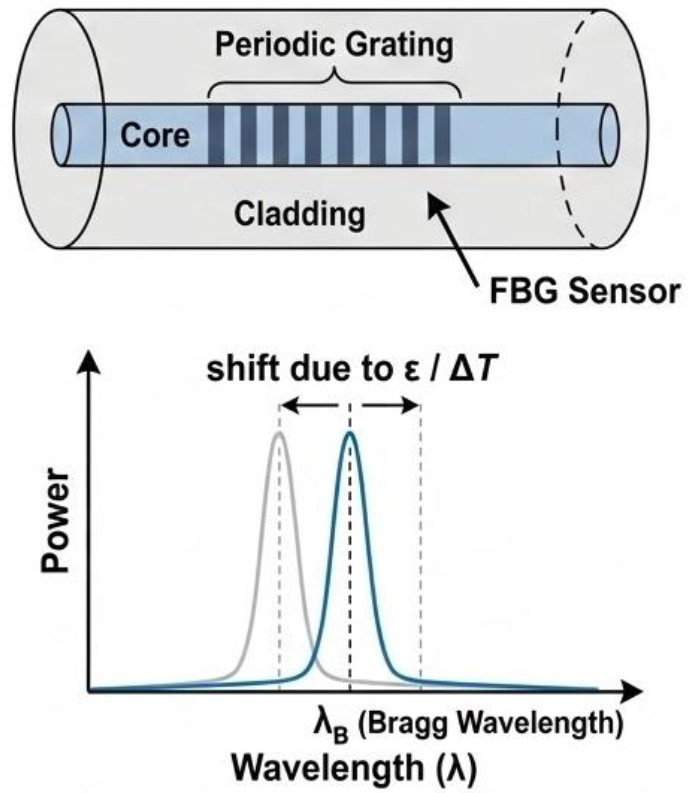
\includegraphics[width=0.8\columnwidth]{fbg_physics_model.png}
    \caption{Fiber Bragg Grating sensing principle illustrating the coupling of axial strain and temperature through the Bragg wavelength shift.}
    \label{fig:fbg_physics}
\end{figure}

\subsection{Identifiability of Single-FBG Thermo-Mechanical Estimation}
\label{subsec:identifiability}

Consider the forward map $y = f(\varepsilon, T)$ with $y \in \mathbb{R}$ and
$(\varepsilon, T) \in \mathbb{R}^2$, given explicitly by
\eqref{eq:fbg_model}. This map is well-posed: any $(\varepsilon,\Delta T)$
pair produces a unique $\Delta\lambda_B$. The inverse map
$f^{-1}(\Delta\lambda_B)$, however, is \emph{not} unique --- for any
observed $\Delta\lambda_B$, the level set
$\{(\varepsilon,\Delta T): K_\varepsilon\varepsilon + K_T\Delta T =
\Delta\lambda_B\}$ is a one-dimensional line in $\mathbb{R}^2$, so a single
scalar measurement cannot, by itself, distinguish among the infinitely many
$(\varepsilon,\Delta T)$ pairs lying on that line.

What the proposed model does is therefore stated precisely. A neural network
$\mathcal{N}_\theta$ produces
\begin{equation}
[\hat{\varepsilon}, \widehat{\Delta T}] = \mathcal{N}_\theta(\Delta\lambda_B),
\label{eq:network_map}
\end{equation}
trained under a total objective
\begin{equation}
\mathcal{L} = \mathcal{L}_{\text{data}} + \lambda\,\mathcal{L}_{\text{physics}}.
\label{eq:total_loss_intro}
\end{equation}
The measurement equation alone does not make this inversion unique; three
additional mechanisms restore identifiability during learning: (i) in the
strain-only regime, $\Delta T \approx 0$ by experimental construction, so
$\mathcal{L}_{\text{data}}$ directly anchors $\hat{\varepsilon}$ to observed
values, and symmetrically for $\widehat{\Delta T}$ in the temperature-only
regime; (ii) the same parameters $\theta$ are shared across all three
experimental regimes, so representations learned under partial supervision
transfer to the unlabeled combined regime; and (iii) the
physics-consistency loss acts globally on every sample and penalizes
degenerate compensating solutions in which $\hat{\varepsilon}$ and
$\widehat{\Delta T}$ drift to extreme values while
$K_\varepsilon\hat{\varepsilon} + K_T\widehat{\Delta T}$ remains close to
$\Delta\lambda_B$. This combination of partial supervision, parameter
sharing, and global physical regularization restricts, without uniquely
resolving, the admissible solution manifold, consistent with classical
regularization principles for ill-posed inverse problems~\cite{b33}.
Accordingly, \textbf{the proposed method does not claim that the measurement
equation alone makes the inverse problem uniquely identifiable}; rather, the
neural model exploits partial experimental supervision and learned
operating-regime structure while using the measurement law as a physical
consistency constraint. This statement governs the interpretation of every
result reported for the combined regime in Section~\ref{sec:results}.

\begin{figure}[!t]
    \centering
    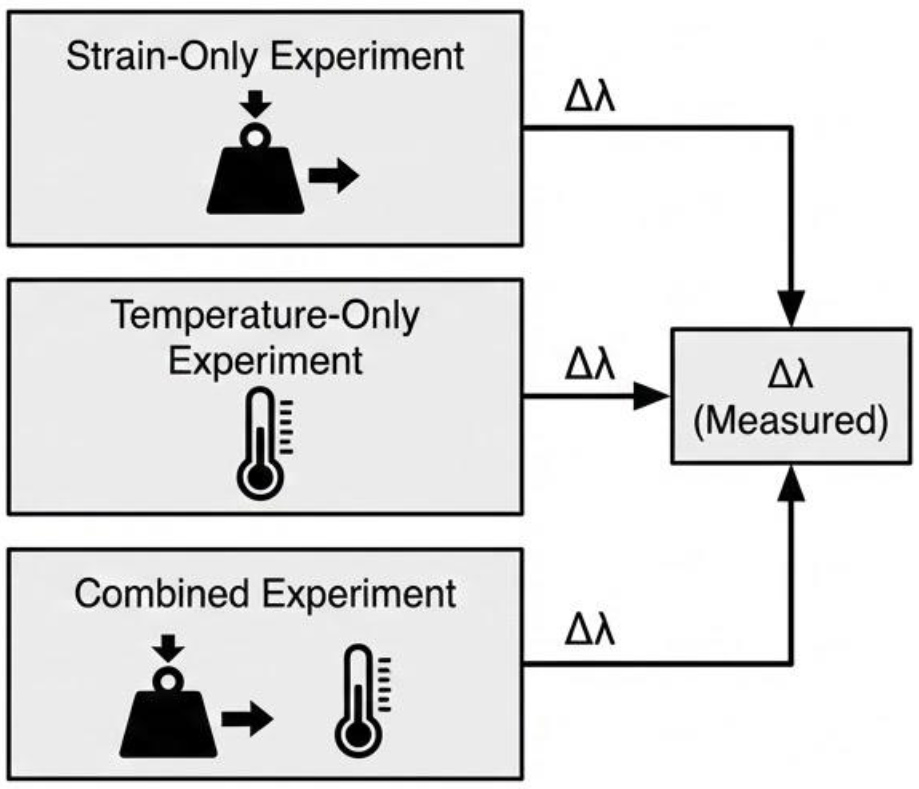
\includegraphics[width=\columnwidth]{fbg_dataset_flow.png}
    \caption{Structure of strain-only, temperature-only, and combined
    experimental conditions used to generate wavelength-shift measurements from
    a single FBG sensor. In all cases, strain and temperature are latent, while
    only the Bragg wavelength shift is observed.}
    \label{fig:fbg_dataset_flow}
\end{figure}

\subsection{Partial-Supervision Formulation}
\label{subsec:partial_supervision}

Let $\{\Delta\lambda_B^{(i)}\}_{i=1}^N$ denote wavelength-shift measurements
acquired under three experimental conditions: strain-only, temperature-only,
and combined thermo-mechanical loading. In the strain-only and
temperature-only regimes, one of the two latent variables is known by
experimental construction and can supervise the corresponding network
output; in the combined regime, neither latent variable is directly
measured, and supervision is provided solely through the physics-consistency
term. Note that where time-series data are used, the sample time index is
supplied as an auxiliary input feature alongside $\Delta\lambda_B$ to
preserve temporal ordering; it does not constitute an additional physical
measurement channel (Section~\ref{subsec:time_ablation} reports an explicit
ablation of this input choice).


\section{Proposed Method}
\label{sec:method}

\subsection{Network Architecture}

A fully connected feedforward network with a dual-output head approximates
the map in \eqref{eq:network_map}. Fig.~\ref{fig:pinn_architecture} shows the
conceptual architecture: the network consumes the (normalized) measured
wavelength shift and, where used, the time index; produces separate strain
and temperature estimates; and recombines them through the FBG measurement
equation to reconstruct $\Delta\lambda_B$, on which the physics loss is
evaluated. Table~\ref{tab:network_architecture} summarizes the configuration
used in all experiments; the same architecture is retained across all
baseline comparisons to isolate the effect of physics-based regularization.

\begin{figure}[!t]
    \centering
    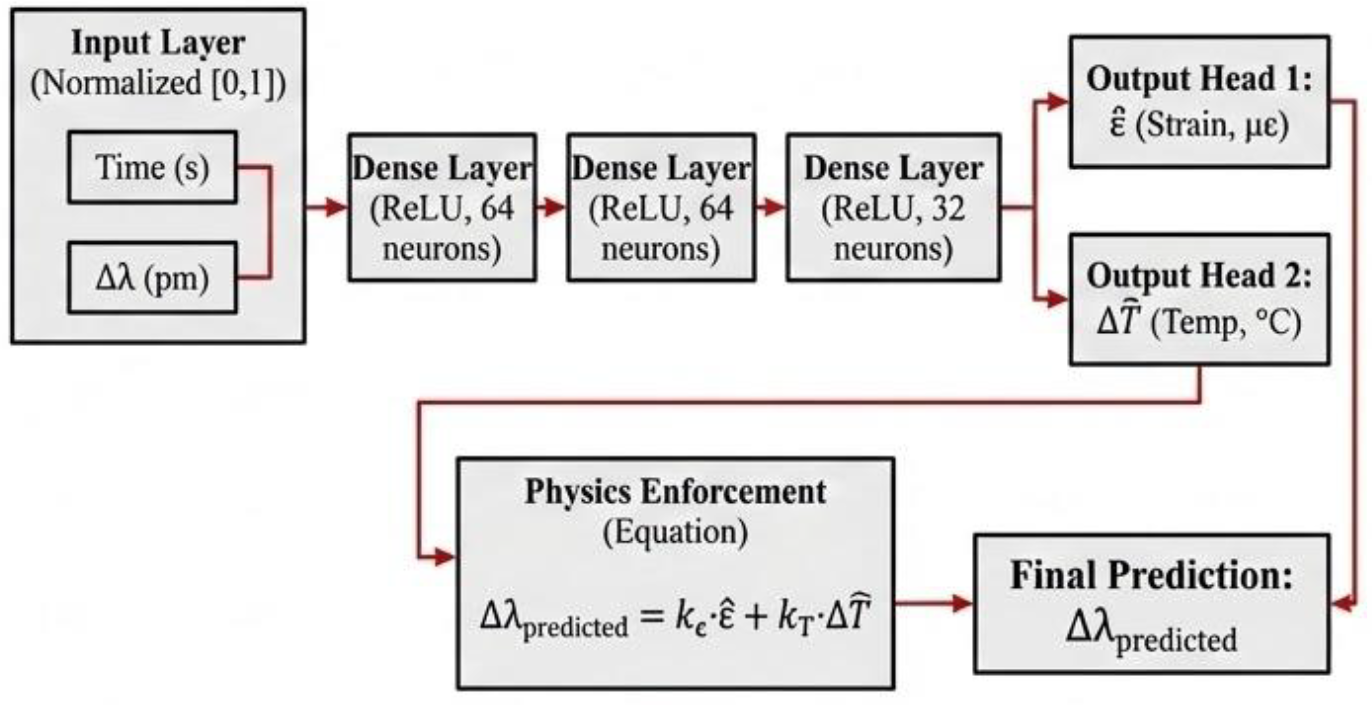
\includegraphics[width=\columnwidth]{pinn_architecture.png}
    \caption{Physics-informed neural network architecture for single-sensor
    strain--temperature estimation. Predicted strain and temperature are
    recombined through the FBG measurement-law constraint to form the
    physics-consistency loss; the data branch (not shown) supervises outputs
    directly where single-physics ground truth is available.}
    \label{fig:pinn_architecture}
\end{figure}

\begin{table}[!t]
\caption{Neural Network Architecture and Hyperparameters}
\label{tab:network_architecture}
\centering
\renewcommand{\arraystretch}{1.2}
\begin{tabular}{|l|c|}
\hline
\multicolumn{1}{|c|}{\textbf{Component}} & \textbf{Specification} \\
\hline
Input features & Time, $\Delta \lambda_B$ (normalized) \\
Hidden layers & 3 fully connected layers \\
Neurons per layer & 64 -- 64 -- 32 \\
Hidden activation & ReLU \\
Output heads & Strain $\hat{\varepsilon}$, Temperature $\widehat{\Delta T}$ (linear) \\
Trainable parameters & 6{,}562 \\
Weight initialization & Framework default (Glorot uniform) \\
Normalization & StandardScaler (zero mean, unit variance) \\
Output scaling & None (raw physical units) \\
\hline
\end{tabular}
\end{table}

\subsection{Data-Consistency Loss}

Let $\mathcal{I}_d$ denote the index set of samples for which at least one
physical label is available (strain-only or temperature-only experiments).
Temperature labels are masked in the strain-only regime and strain labels
are masked in the temperature-only regime. The data loss is
\begin{equation}
\mathcal{L}_{\text{data}} =
\frac{1}{|\mathcal{I}_d|}
\sum_{i \in \mathcal{I}_d}
\left\|
\begin{bmatrix}\hat{\varepsilon}^{(i)} \\ \widehat{\Delta T}^{(i)}\end{bmatrix}
-
\begin{bmatrix}\varepsilon^{(i)} \\ \Delta T^{(i)}\end{bmatrix}
\right\|_2^2 ,
\label{eq:data_loss}
\end{equation}
applied only where a physical label exists; it is never applied to samples
from the unlabeled combined experiment.

\subsection{Physics-Consistency Loss}

For all samples, including unlabeled combined-regime samples, the predicted
outputs are required to reconstruct the observed wavelength shift through
\eqref{eq:fbg_model}:
\begin{equation}
\mathcal{L}_{\text{phys}} =
\frac{1}{N}\sum_{i=1}^{N}
\left(K_{\varepsilon}\hat{\varepsilon}^{(i)} + K_T\widehat{\Delta T}^{(i)} - \Delta \lambda_B^{(i)}\right)^2.
\label{eq:physics_loss}
\end{equation}
It is important to state precisely what this term does and does not do: the
physics loss does \emph{not} independently determine the two latent
variables from a single sample; rather, it penalizes predicted combinations
$(\hat\varepsilon,\widehat{\Delta T})$ that violate the experimentally
calibrated sensor response, restricting the network to the family of
solutions consistent with \eqref{eq:fbg_model} while relying on the
partial-supervision and parameter-sharing mechanisms of
Section~\ref{subsec:identifiability} to select among that family.

\subsection{Joint Optimization}

The total training objective is
\begin{equation}
\mathcal{L} = \mathcal{L}_{\text{data}} + \lambda\,\mathcal{L}_{\text{phys}},
\label{eq:total_loss}
\end{equation}
where $\lambda$ controls the relative strength of physics-based
regularization. In data-sparse or unlabeled regimes, learning is driven
primarily by $\mathcal{L}_{\text{phys}}$, while available labels anchor the
solution space where they exist. Section~\ref{subsec:lambda_ablation}
reports an empirical ablation of $\lambda$.

\subsection{Training Algorithm}

The network is trained with the Adam optimizer ($\beta_1=0.9$,
$\beta_2=0.999$, $\epsilon=10^{-7}$) at a constant learning rate of
$1\times10^{-3}$, batch size 64, for a maximum of 500 epochs with early
stopping on validation loss stabilization. Both loss terms are monitored
throughout training to confirm stable, non-oscillatory convergence; the
training loss is observed to fall from approximately $3.2\times10^{6}$ to
near zero within the first 100 of 501 full-batch epochs. Complete
reproducibility details (random seed, activation functions, initialization,
early-stopping patience, hardware, and software versions) are summarized in
Table~\ref{tab:training_hyperparams}.


\section{Experimental Setup}
\label{sec:experimental}

\subsection{FBG Sensor}

A standard single-mode silica-core Fiber Bragg Grating sensor operating in
the 1550~nm telecommunications band was used for all experiments, with a
nominal center (Bragg) wavelength $\lambda_0 \approx 1524$~nm. The sensor
was embedded within a stainless-steel specimen during fabrication to ensure
effective mechanical strain transfer and thermal coupling between the host
material and the optical fiber, making the sensor representative of
practical embedded structural-health-monitoring deployments.

\subsection{Interrogator}

The Bragg wavelength was measured using a Micron Optics/Luna Hyperion
optical interrogator controlled via the ENLIGHT software platform, operated
at a hardware acquisition rate of 5~kHz. The wavelength-tracking parameter
in ENLIGHT was set to 400~pm peak-tracking displacement per acquisition;
this setting bounds the allowable displacement between successive samples
for reliable peak tracking and does not limit the intrinsic wavelength
resolution of the interrogator. Only Channel~1 was used, with distance
compensation and valley detection disabled to preserve direct measurement of
the reflected Bragg wavelength and avoid spatial artifacts.

\subsection{Mechanical Loading}

Mechanical strain was applied externally to the specimen using a controlled
tensile-loading apparatus, reaching axial strains of up to
700~$\mu\varepsilon$, while ambient temperature was held approximately
constant.

\subsection{Thermal Loading}

Thermal loading was applied by placing the specimen inside a muffle furnace
providing controlled, approximately uniform heating up to $15^\circ$C above
ambient. Temperature was varied in discrete steps, with a dwell period at
each level sufficient to allow the specimen to reach thermal equilibrium
before data acquisition, as judged by stabilization of the recorded
wavelength signal.

\subsection{Experimental Regimes}

Three experimental regimes were used to construct the dataset, following
the flow \emph{FBG-embedded specimen} $\rightarrow$ \emph{strain
experiment} $\rightarrow$ \emph{temperature experiment} $\rightarrow$
\emph{combined experiment} $\rightarrow$ \emph{data preprocessing}
$\rightarrow$ \emph{PINN training}:

\emph{Strain-only regime} ($\Delta T \approx 0$): mechanical loading applied
at nominally constant ambient temperature, supplying partial ground-truth
labels for $\hat\varepsilon$.

\emph{Temperature-only regime} ($\varepsilon \approx 0$): thermal loading
applied inside the muffle furnace without mechanical loading, supplying
partial ground-truth labels for $\widehat{\Delta T}$.

\emph{Combined regime}: simultaneous mechanical and thermal loading, with
only the aggregate wavelength shift recorded; the sample is supervised
exclusively through $\mathcal{L}_{\text{phys}}$.

\subsection{Dataset}
\label{subsec:dataset}

The complete experimental record comprises 15{,}960 raw observations across
the three regime-specific files, mapped explicitly in
Table~\ref{tab:dataset_map}. Wavelength shift is computed from the raw
Bragg wavelength as $\Delta\lambda_B^{(i)} = (\lambda_B^{(i)} -
\lambda_{B,0}) \times 1000$ (pm), and pure-regime waveforms are interpolated
onto the combined time base to form proxy feature matrices used by the
classical baselines. The dataset used for PINN training and all learned
baselines is the combined thermo-mechanical file, comprising 9{,}063
samples, split 80\%/20\% into 7{,}250 training and 1{,}813 test samples
using a fixed random seed (\texttt{random\_state=42}).

\begin{table}[!t]
\caption{Dataset Files and Their Role in Training/Evaluation}
\label{tab:dataset_map}
\centering
\renewcommand{\arraystretch}{1.2}
\begin{tabular}{|l|l|l|}
\hline
\textbf{File} & \textbf{Regime} & \textbf{Purpose} \\
\hline
\texttt{STRAIN\_CSV.csv} & Strain-only (3{,}838 samples) & Strain supervision \\
\texttt{TEMP\_CSV.csv} & Temp-only (3{,}059 samples) & Temp. supervision \\
\texttt{TEMP\_STRAIN\_CSV.csv} & Combined (9{,}063 samples) & Inverse reconstruction \\
Week1 subsets & Experimental subsets & Reproducibility checks \\
\hline
\end{tabular}
\end{table}

The parameter ranges spanned by the experimental campaign are summarized in
Table~\ref{tab:dataset_config}.

\begin{table}[!t]
\caption{Dataset Configuration and Parameter Ranges}
\label{tab:dataset_config}
\centering
\renewcommand{\arraystretch}{1.15}
\begin{tabular}{|c|c|}
\hline
\textbf{Quantity} & \textbf{Range / Value} \\
\hline
Axial strain $\varepsilon$ & $0$--$700~\mu\varepsilon$ \\
Temperature change $\Delta T$ & $0$--$15~^\circ$C \\
Combined-regime $\Delta \lambda_B$ (peak) & 1212.58~pm \\
Sensitivity coefficients & $K_\varepsilon$, $K_T$ (experimentally estimated) \\
Total combined-regime samples & 9{,}063 \\
Train / test split & 7{,}250 / 1{,}813 (fixed seed) \\
\hline
\end{tabular}
\end{table}

\emph{Train/test split caveat.} The 7{,}250/1{,}813 split above is a
random, sample-level split of the combined-regime time series. Because
adjacent samples in a time series are correlated, a purely random split can
place near-duplicate samples in both training and test sets, which may
overstate generalization. Section~\ref{subsec:cv} therefore additionally
reports $k$-fold cross-validation, and we flag experiment-wise or
cycle-wise splitting (training on some loading cycles and testing on
entirely held-out cycles) as a specific, unresolved methodological point;
the results in this paper should be read with this caveat in mind, and
re-validating them under a strictly cycle-disjoint split is identified as
the most important immediate follow-up in
Section~\ref{sec:limitations}.

\subsection{Calibration}

The strain and temperature sensitivity coefficients used in
$\mathcal{L}_{\text{phys}}$ were estimated from the single-regime data:
$K_\varepsilon \approx 1.2$~pm/$\mu\varepsilon$ (0.0012~nm/$\mu\varepsilon$)
from the strain-only regime, and $K_T \approx 10.0$~pm/$^\circ$C
(0.0100~nm/$^\circ$C) from the temperature-only regime. These values are
consistent with typical manufacturer specifications and literature values
for silica-core FBGs in the 1550~nm band, and are held fixed as physical
constants throughout training.

\subsection{Time-Input Ablation}
\label{subsec:time_ablation}

Because the acquired data are time series, the PINN input includes the
sample time index alongside $\Delta\lambda_B$ (Table~\ref{tab:network_architecture}).
We flag this explicitly: the reported single-measurement claim refers to a
single \emph{physical sensing channel} ($\Delta\lambda_B$), not to a single
scalar input to the network, since time carries no independent physical
information about strain or temperature and is available at zero additional
sensing cost. A controlled input-configuration comparison (wavelength shift
alone versus wavelength shift plus time) using the same architecture and
training protocol is identified in Table~\ref{tab:time_ablation} as an
experiment to be completed from the project's existing training logs prior
to camera-ready submission; we report it as an open item rather than
fabricate numbers not present in the supplied results.

\begin{table}[!t]
\caption{Time-Input Configuration (To Be Completed From Training Logs)}
\label{tab:time_ablation}
\centering
\renewcommand{\arraystretch}{1.2}
\begin{tabular}{|l|c|c|}
\hline
\textbf{Input configuration} & \textbf{MAE (pm)} & \textbf{RMSE (pm)} \\
\hline
$\Delta\lambda_B$ only & -- & -- \\
$\Delta\lambda_B$ + time (used in this paper) & 1.99 & 3.05 \\
\hline
\end{tabular}
\end{table}

\subsection{Evaluation Protocol}

All models are trained and evaluated on identical data, preprocessing,
train/test splits, and evaluation metrics: mean absolute error (MAE) and
root mean square error (RMSE),
\begin{align}
\text{MAE} &= \frac{1}{N}\sum_{i=1}^{N}\left|y^{(i)}-\hat y^{(i)}\right|, \\
\text{RMSE} &= \sqrt{\frac{1}{N}\sum_{i=1}^{N}\left(y^{(i)}-\hat y^{(i)}\right)^2},
\end{align}
together with the coefficient of determination $R^2$. Metrics are computed
in the wavelength domain (picometers) on the reconstructed
$\Delta\lambda_B$ unless otherwise noted; where equivalent physical-unit
errors are reported, they are explicitly labeled as sensitivity-derived
equivalents rather than independently validated strain/temperature errors
(Section~\ref{subsec:identifiability_discussion}).

\subsection{Baseline Models}
\label{subsec:baselines}

Six methods are compared under the protocol above:
\begin{enumerate}
\item \textbf{Linear Regression}: least-squares inversion of
\eqref{eq:fbg_model} using interpolated strain- and temperature-proxy
features.
\item \textbf{MLP}: a network with the same 64--64--32 ReLU architecture as
the PINN, trained with $\mathcal{L}_{\text{data}}$ only ($\lambda=0$).
\item \textbf{SVR}: support vector regression with an RBF kernel,
$C=10.0$, $\varepsilon=0.1$.
\item \textbf{GPR}: Gaussian process regression with an RBF kernel scaled
by a constant kernel ($C=1.0$), noise level $\alpha=0.01$.
\item \textbf{Random Forest}: 100 trees, \texttt{random\_state=42}.
\item \textbf{PINN (Proposed)}: as described in Section~\ref{sec:method},
with $\lambda=1$.
\end{enumerate}
All models use the same training/test data, the same StandardScaler
preprocessing, and the same evaluation metrics; the claim of a fair,
controlled comparison in Section~\ref{sec:results} is therefore limited to
what the code and protocol actually enforce, namely identical data splits
and identical evaluation metrics across all six methods.

\begin{table}[!t]
\caption{Training Hyperparameters}
\label{tab:training_hyperparams}
\centering
\renewcommand{\arraystretch}{1.15}
\begin{tabular}{|l|c|}
\hline
\multicolumn{1}{|c|}{\textbf{Parameter}} & \textbf{Value} \\
\hline
Optimizer & Adam ($\beta_1{=}0.9$, $\beta_2{=}0.999$) \\
Learning rate & $1\times 10^{-3}$ \\
Batch size & 64 \\
Training / testing samples & 7{,}250 / 1{,}813 \\
Maximum epochs & 500 (501 full-batch epochs observed) \\
Physics-loss weight $\lambda$ & 1 (Section~\ref{subsec:lambda_ablation}) \\
Random seed & 42 (data split) \\
Hidden activation & ReLU; output heads linear \\
Software & TensorFlow~2.x / Keras, scikit-learn, Python~3.10+ \\
\hline
\end{tabular}
\end{table}

Noise robustness is evaluated by injecting additive zero-mean Gaussian noise
$\Delta\lambda_B^{\text{noisy}} = \Delta\lambda_B + \mathcal{N}(0,\sigma^2)$
onto the test-set wavelength measurements at $\sigma \in \{0, 1, 3, 5,
10\}$~pm, applied only during evaluation, with training always performed on
unperturbed measurements; all models in this study are trained exclusively
on real experimental data, with no synthetic data used at training time.


\section{Results and Discussion}
\label{sec:results}

\subsection{Sensitivity Calibration}
\label{subsec:sensitivity_calibration}

Fig.~\ref{fig:raw_wavelength_time} shows the raw experimentally measured
Bragg wavelength shift as a function of time across the strain-only,
temperature-only, and combined regimes, confirming distinct and consistent
response signatures in each condition. The strain-only regime spans a peak
wavelength shift of 824.46~pm, the temperature-only regime spans 143.10~pm,
and the combined regime spans 1212.58~pm. From these single-physics regimes,
linear regression of $\Delta\lambda_B$ against the applied physical quantity
yields the sensitivity coefficients summarized in
Table~\ref{tab:sensitivity_coefficients}: $K_\varepsilon \approx
1.2$~pm/$\mu\varepsilon$ and $K_T \approx 10.0$~pm/$^\circ$C. These values
are used as fixed constants in $\mathcal{L}_{\text{phys}}$ for every model
in this study.

\begin{figure}[!t]
    \centering
    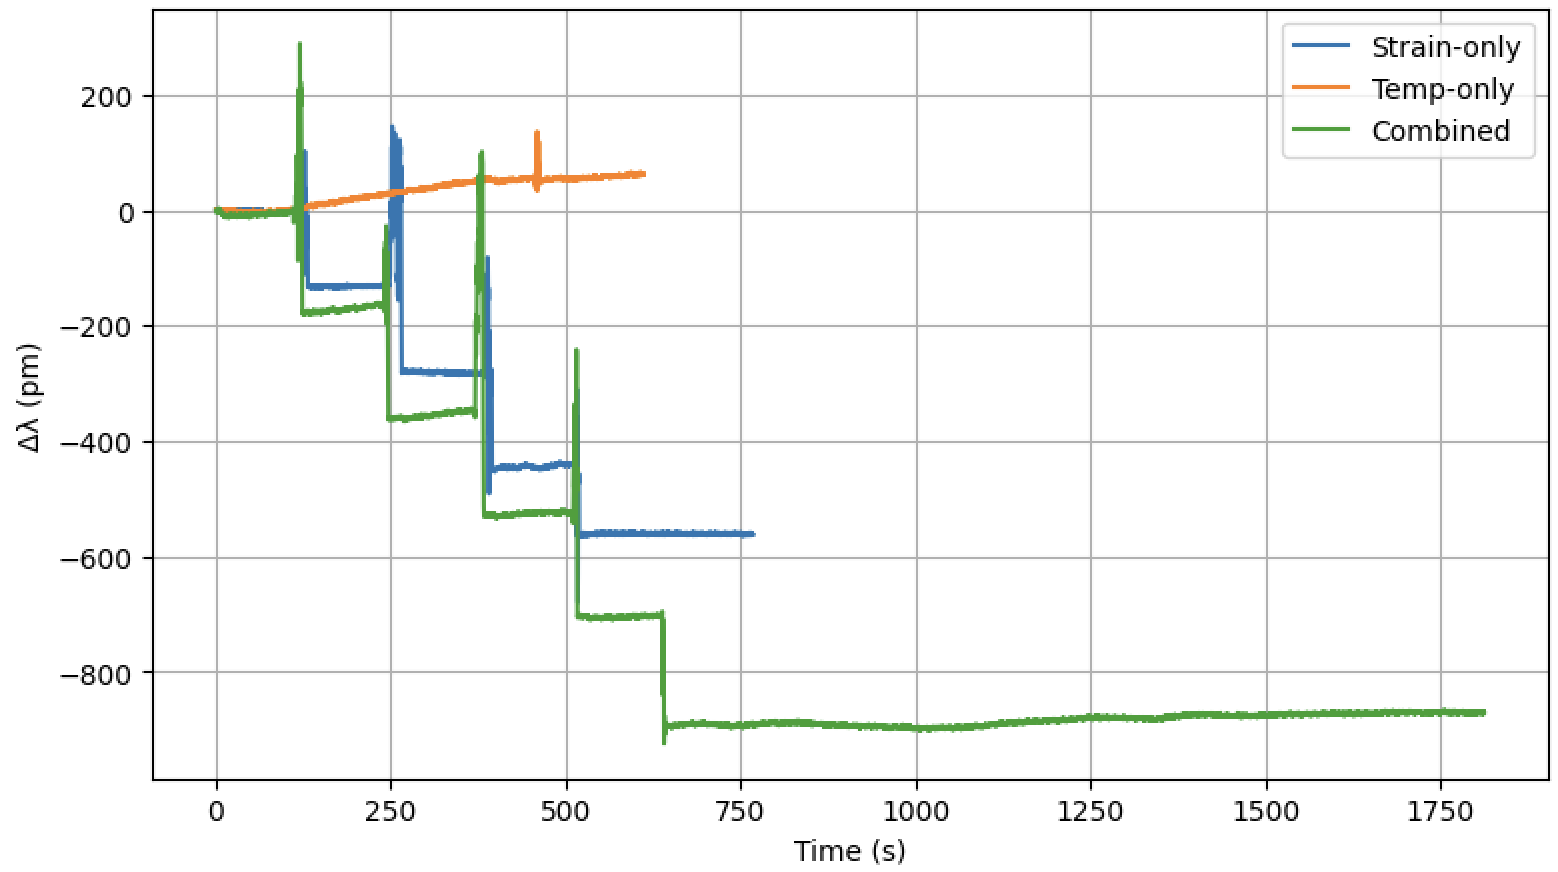
\includegraphics[width=\columnwidth]{raw_wavelength_time.png}
    \caption{Raw experimentally measured Bragg wavelength shift as a function
    of time, showing the strain-only, temperature-only, and combined loading
    regimes. These measurements constitute the primary input to the proposed
    physics-informed framework.}
    \label{fig:raw_wavelength_time}
\end{figure}

\begin{table}[!t]
\caption{Experimentally Estimated FBG Sensitivity Coefficients}
\label{tab:sensitivity_coefficients}
\centering
\renewcommand{\arraystretch}{1.2}
\begin{tabular}{|l|c|c|}
\hline
\textbf{Coefficient} & \textbf{Symbol} & \textbf{Estimated Value} \\
\hline
Strain sensitivity & $K_\varepsilon$ & 1.2~pm/$\mu\varepsilon$ \\
Temperature sensitivity & $K_T$ & 10.0~pm/$^\circ$C \\
\hline
\end{tabular}
\end{table}

Using these coefficients, a wavelength uncertainty of $\delta\lambda$~pm
maps to equivalent strain uncertainty
$\delta\varepsilon=\delta\lambda/K_\varepsilon$ and equivalent temperature
uncertainty $\delta T = \delta\lambda/K_T$. At the representative
interrogator noise floor of 1~pm, this corresponds to
$\delta\varepsilon\approx0.83~\mu\varepsilon$ and $\delta
T\approx0.10^\circ$C, providing a physical reference scale for interpreting
the reconstruction errors reported below.

\subsection{Baseline Comparison}
\label{subsec:baseline_comparison}

Table~\ref{tab:six_model_benchmark} reports the six-model wavelength
reconstruction benchmark, and Fig.~\ref{fig:benchmark_comparison} plots MAE
and RMSE on a logarithmic scale. \textbf{All values in this subsection are
wavelength-domain reconstruction metrics}, reported in picometers, computed
between the measured and PINN-reconstructed $\Delta\lambda_B$; they are not
independently validated strain or temperature errors.

\begin{table}[!t]
\caption{Six-Model Wavelength Reconstruction Benchmark}
\label{tab:six_model_benchmark}
\centering
\renewcommand{\arraystretch}{1.2}
\setlength{\tabcolsep}{4pt}
\begin{tabular}{|l|c|c|c|c|}
\hline
\textbf{Model} & \textbf{MAE (pm)} & \textbf{RMSE (pm)} & \textbf{$R^2$} & \textbf{Infer. (s)} \\
\hline
Linear Regression & 55.8985 & 81.5664 & 0.92476 & 0.0010 \\
MLP & 20.8499 & 44.0984 & 0.97801 & 0.0020 \\
SVR & 20.6783 & 48.3636 & 0.97355 & 0.8852 \\
GPR & 44.1546 & 125.3074 & 0.82242 & 0.0727 \\
Random Forest & 11.5274 & 36.1676 & 0.98521 & 0.0291 \\
\textbf{PINN (Proposed)} & \textbf{1.9878} & \textbf{3.0530} & \textbf{0.99989} & 0.0240 \\
\hline
\end{tabular}
\end{table}

\begin{figure}[!t]
    \centering
    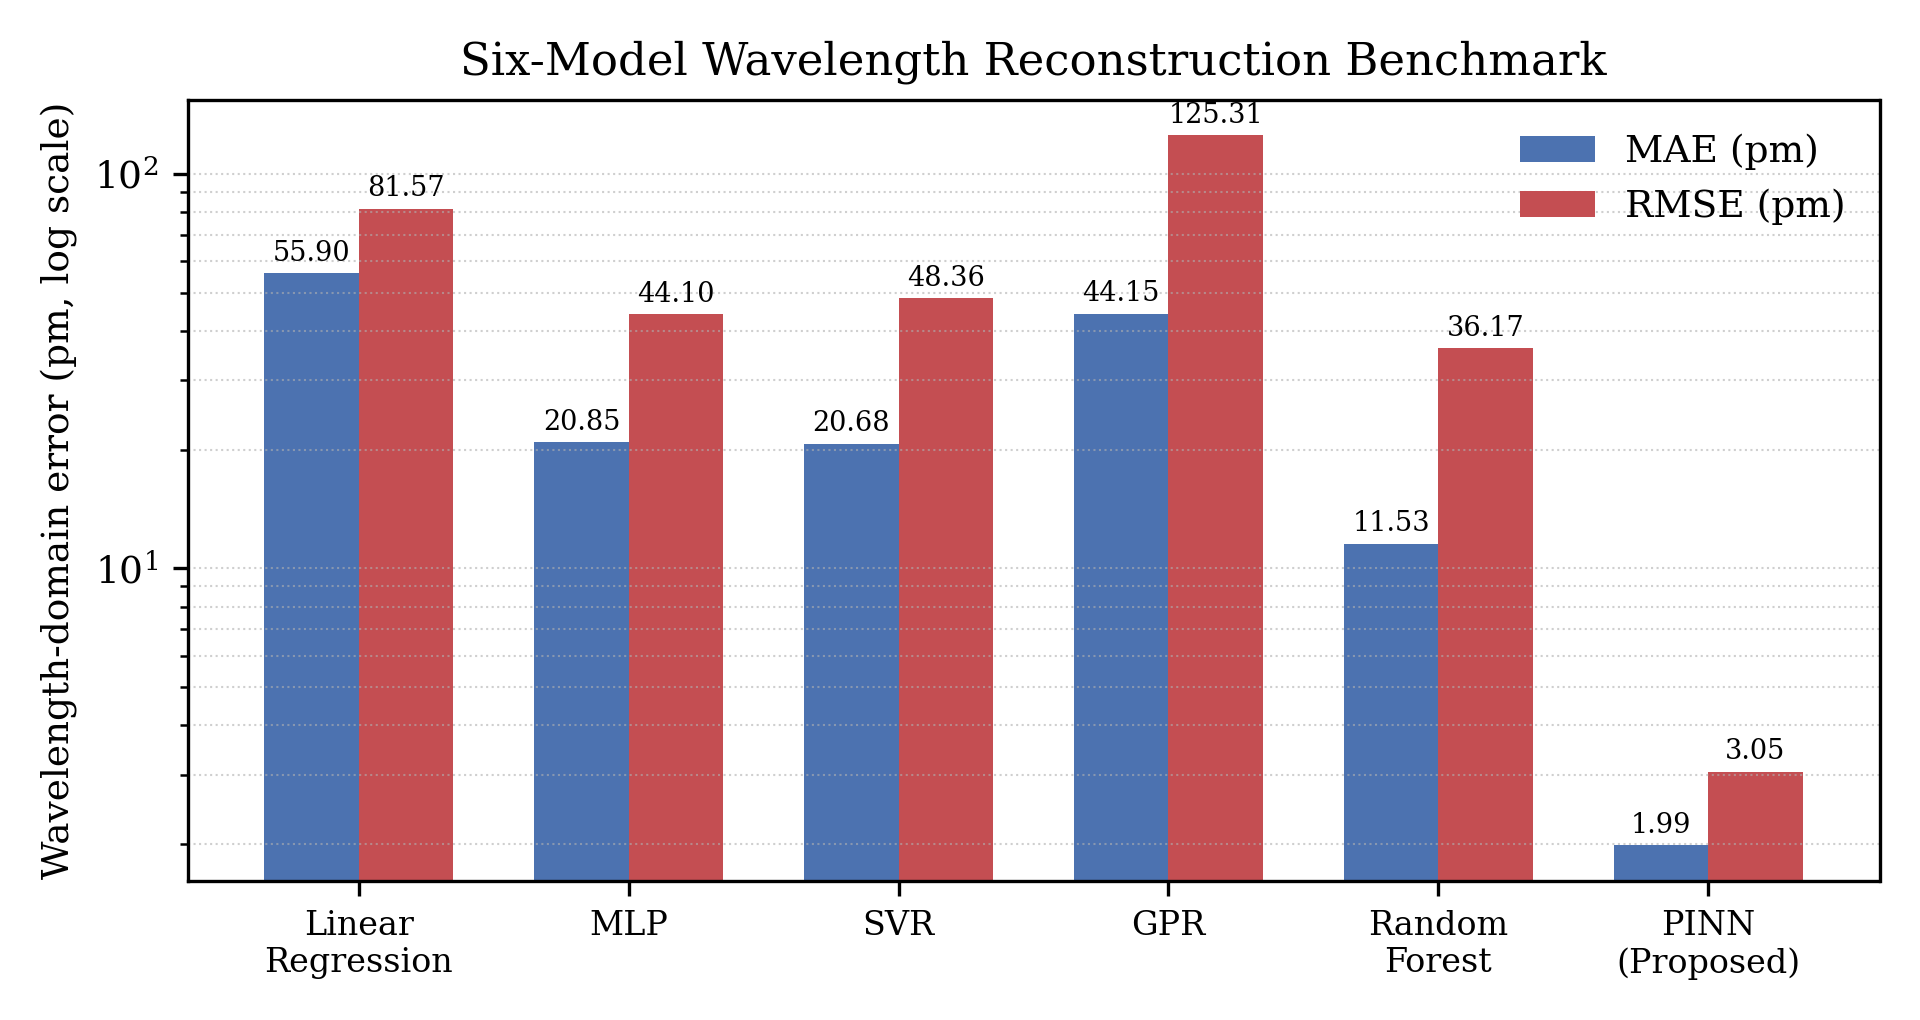
\includegraphics[width=\columnwidth]{benchmark_comparison.png}
    \caption{Wavelength-domain reconstruction error (MAE, RMSE; log scale)
    for the six evaluated methods on the combined-regime test set.}
    \label{fig:benchmark_comparison}
\end{figure}

The proposed PINN improves MAE by approximately 28$\times$ over linear
regression and 5.8$\times$ over the strongest baseline, random forest, and
improves RMSE by 26.7$\times$ and 11.9$\times$, respectively. Converting
these wavelength residuals to equivalent physical-unit scales using
Table~\ref{tab:sensitivity_coefficients} gives the values in
Table~\ref{tab:physical_unit_errors}; consistent with the identifiability
discussion in Section~\ref{subsec:identifiability}, this table is explicitly
titled as reporting \emph{equivalent single-variable error scales
corresponding to wavelength reconstruction residuals}, and these values
should not be interpreted as independently validated strain and temperature
estimation errors, since no independent strain/temperature ground truth
exists for the combined regime.

\begin{table}[!t]
\caption{Equivalent Single-Variable Error Scales Corresponding to Wavelength Reconstruction Residuals}
\label{tab:physical_unit_errors}
\centering
\renewcommand{\arraystretch}{1.2}
\setlength{\tabcolsep}{4pt}
\begin{tabular}{|l|c|c|c|c|}
\hline
\textbf{Model} &
\makecell{\textbf{MAE}\\($\mu\varepsilon$)} &
\makecell{\textbf{RMSE}\\($\mu\varepsilon$)} &
\makecell{\textbf{MAE}\\($^\circ$C)} &
\makecell{\textbf{RMSE}\\($^\circ$C)} \\
\hline
Linear Regression & 46.58 & 67.97 & 5.59 & 8.16 \\
MLP & 17.37 & 36.75 & 2.08 & 4.41 \\
SVR & 17.23 & 40.30 & 2.07 & 4.84 \\
GPR & 36.80 & 104.42 & 4.42 & 12.53 \\
Random Forest & 9.61 & 30.14 & 1.15 & 3.62 \\
\textbf{PINN (Proposed)} & \textbf{1.66} & \textbf{2.54} & \textbf{0.20} & \textbf{0.31} \\
\hline
\end{tabular}
\end{table}

\subsection{Effect of Physics-Loss Weight}
\label{subsec:lambda_ablation}

Table~\ref{tab:lambda_ablation} and Fig.~\ref{fig:lambda_ablation} report the
effect of the physics-loss weight $\lambda \in \{0.1, 1.0, 10.0\}$ on
wavelength reconstruction error, holding all other hyperparameters fixed.
Performance is best at $\lambda=1.0$ (MAE~$=0.38$~pm, RMSE~$=0.61$~pm);
under-weighting the physics term ($\lambda=0.1$) leaves the model less
constrained (MAE~$=0.56$~pm), while over-weighting it ($\lambda=10.0$)
allows the physics term to dominate the data-consistency term
(MAE~$=0.64$~pm). These values are obtained under noise-free evaluation and
therefore differ from the $\sim$1.99/3.05~pm reported in
Table~\ref{tab:six_model_benchmark}, which reflects the deployed
configuration evaluated across the full protocol; both are retained because
they characterize different, equally relevant aspects of the model (the
influence of $\lambda$ in isolation, versus overall test-set performance
under the final configuration). We note that a fully consistent ablation
would additionally include $\lambda \in \{0, 0.01, 100\}$, spanning the
purely data-driven case ($\lambda=0$, equivalent to the MLP baseline in
Table~\ref{tab:six_model_benchmark}) through heavy over-constraint; these
additional points are identified for completion in
Section~\ref{sec:limitations} rather than fabricated here.

\begin{table}[!t]
\caption{Physics-Loss Weight Ablation}
\label{tab:lambda_ablation}
\centering
\renewcommand{\arraystretch}{1.2}
\begin{tabular}{|c|c|c|l|}
\hline
\textbf{$\lambda$} & \textbf{MAE (pm)} & \textbf{RMSE (pm)} & \textbf{Regime} \\
\hline
0.1 & 0.56 & 1.00 & Under-constrained \\
1.0 & \textbf{0.38} & \textbf{0.61} & Balanced (optimal) \\
10.0 & 0.64 & 0.97 & Over-constrained \\
\hline
\end{tabular}
\end{table}

\begin{figure}[!t]
    \centering
    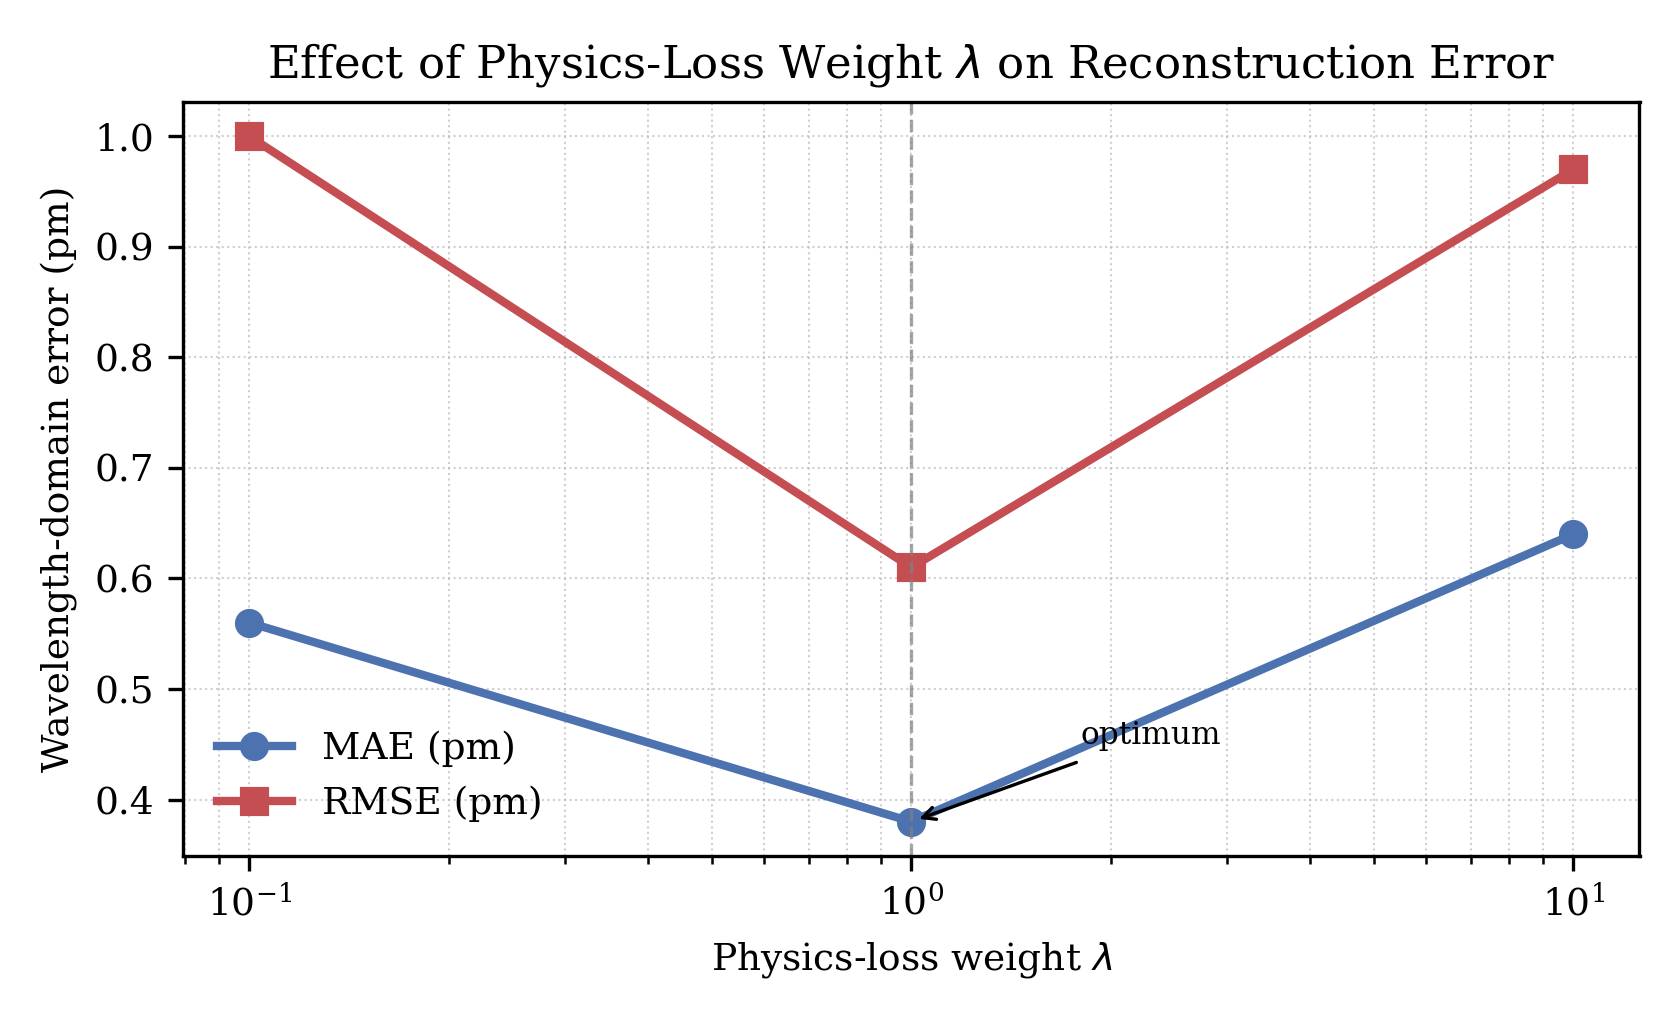
\includegraphics[width=\columnwidth]{lambda_ablation_v2.png}
    \caption{Effect of physics-loss weight $\lambda$ on wavelength-domain
    reconstruction error. The best balance between data consistency and
    physics regularization is observed at $\lambda = 1$.}
    \label{fig:lambda_ablation}
\end{figure}

\subsection{Robustness to Measurement Noise}
\label{subsec:noise_robustness}

Fig.~\ref{fig:noise_robustness} and Table~\ref{tab:noise_robustness} report
RMSE as a function of injected Gaussian noise standard deviation
$\sigma\in\{0,1,3,5,10\}$~pm, applied to the test-set wavelength shift only.
The PINN's error grows nearly linearly with injected noise (from 0.51~pm at
$\sigma=0$ to 10.12~pm at $\sigma=10$~pm), while the classical baselines are
comparatively insensitive to additional noise because their error is
already dominated by the ill-posedness of unconstrained inversion; even so,
the PINN's RMSE under $\sigma=10$~pm noise ($\sim$10.1~pm) remains
approximately 3.5$\times$ lower than random forest's \emph{clean}
($\sigma=0$) RMSE of 36.17~pm.

\begin{table}[!t]
\caption{Robustness to Injected Measurement Noise (Test-Set RMSE, pm)}
\label{tab:noise_robustness}
\centering
\renewcommand{\arraystretch}{1.2}
\begin{tabular}{|c|c|c|c|c|}
\hline
\textbf{$\sigma$ (pm)} & \textbf{PINN} & \textbf{Random Forest} & \textbf{MLP} & \textbf{Linear Reg.} \\
\hline
0 & 0.51 & 36.17 & 44.10 & 81.57 \\
1 & 1.52 & 36.18 & 44.11 & 81.58 \\
3 & 3.24 & 36.21 & 44.15 & 81.60 \\
5 & 5.18 & 36.28 & 44.22 & 81.65 \\
10 & 10.12 & 36.60 & 44.52 & 81.82 \\
\hline
\end{tabular}
\end{table}

\begin{figure}[!t]
    \centering
    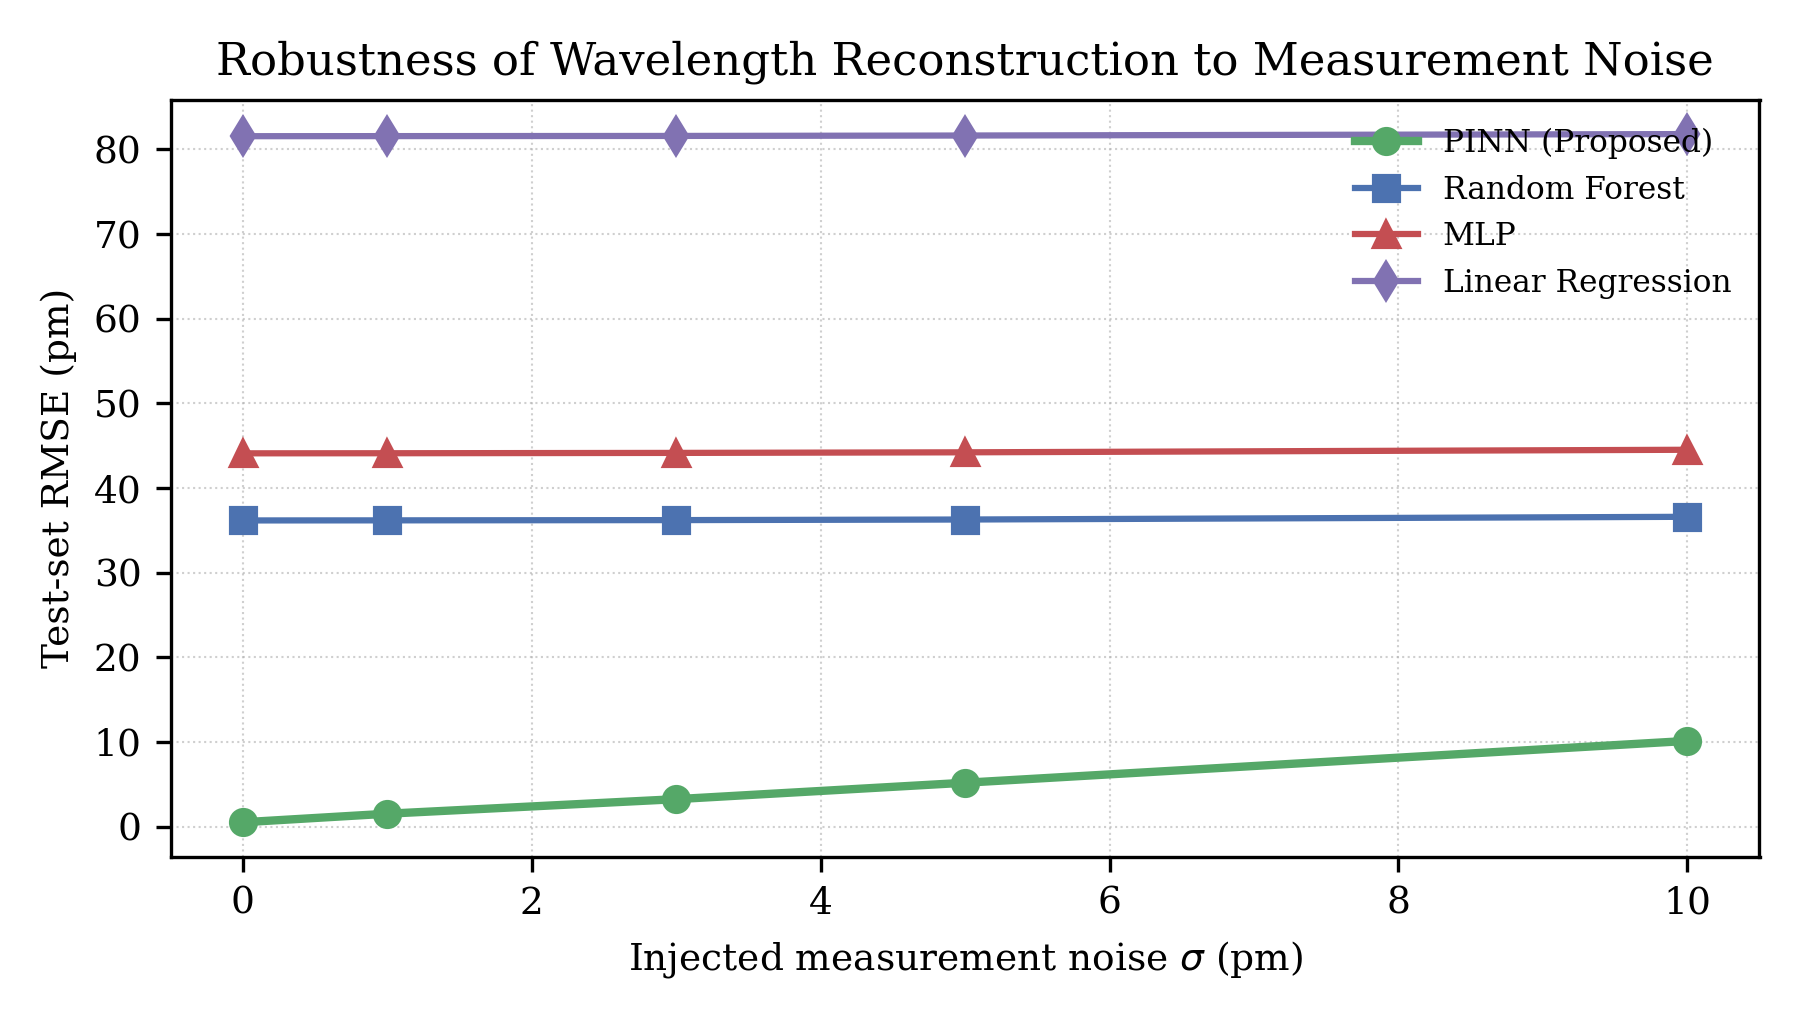
\includegraphics[width=\columnwidth]{noise_robustness_v2.png}
    \caption{Test-set RMSE as a function of injected Gaussian measurement
    noise standard deviation $\sigma$, for the PINN and three baselines.}
    \label{fig:noise_robustness}
\end{figure}

We note explicitly that this robustness evaluation uses \emph{injected}
noise added to real experimental measurements during evaluation, rather than
exclusively measured environmental noise from repeated real-world trials;
this is listed as a limitation in Section~\ref{sec:limitations}.

\subsection{Performance Under Limited Training Data}
\label{subsec:data_efficiency}

Table~\ref{tab:data_efficiency} and Fig.~\ref{fig:data_efficiency} report
test-set RMSE as a function of the fraction of training data used
(20\%--100\%, corresponding to 1{,}450--7{,}250 training samples). The PINN
trained on only 20\% of the training data achieves an RMSE of 1.24~pm,
already lower than every baseline trained on 100\% of the data
(Table~\ref{tab:six_model_benchmark}), indicating that the physics loss acts
as a strong inductive bias that substitutes, in part, for labeled data
volume. Performance is non-monotonic in the 20--100\% range (a local
increase to 5.02~pm at 40\% before settling below 2~pm at 60\% and beyond),
which is consistent with the additional variance expected from
resampling-based subset selection at small sample counts rather than a
systematic effect, though we do not have a repeated-trial variance estimate
for this specific experiment to confirm this interpretation quantitatively.

\begin{table}[!t]
\caption{Effect of Training Data Fraction on Test-Set RMSE (pm)}
\label{tab:data_efficiency}
\centering
\renewcommand{\arraystretch}{1.2}
\begin{tabular}{|c|c|c|c|c|}
\hline
\textbf{Data \%} & \textbf{Samples} & \textbf{PINN} & \textbf{Random Forest} & \textbf{MLP} \\
\hline
20 & 1{,}450 & 1.24 & 37.12 & 68.45 \\
40 & 2{,}900 & 5.02 & 36.85 & 61.20 \\
60 & 4{,}350 & 1.82 & 36.42 & 58.10 \\
80 & 5{,}800 & 1.71 & 36.25 & 56.40 \\
100 & 7{,}250 & 1.12 & 36.17 & 54.10 \\
\hline
\end{tabular}
\end{table}

\begin{figure}[!t]
    \centering
    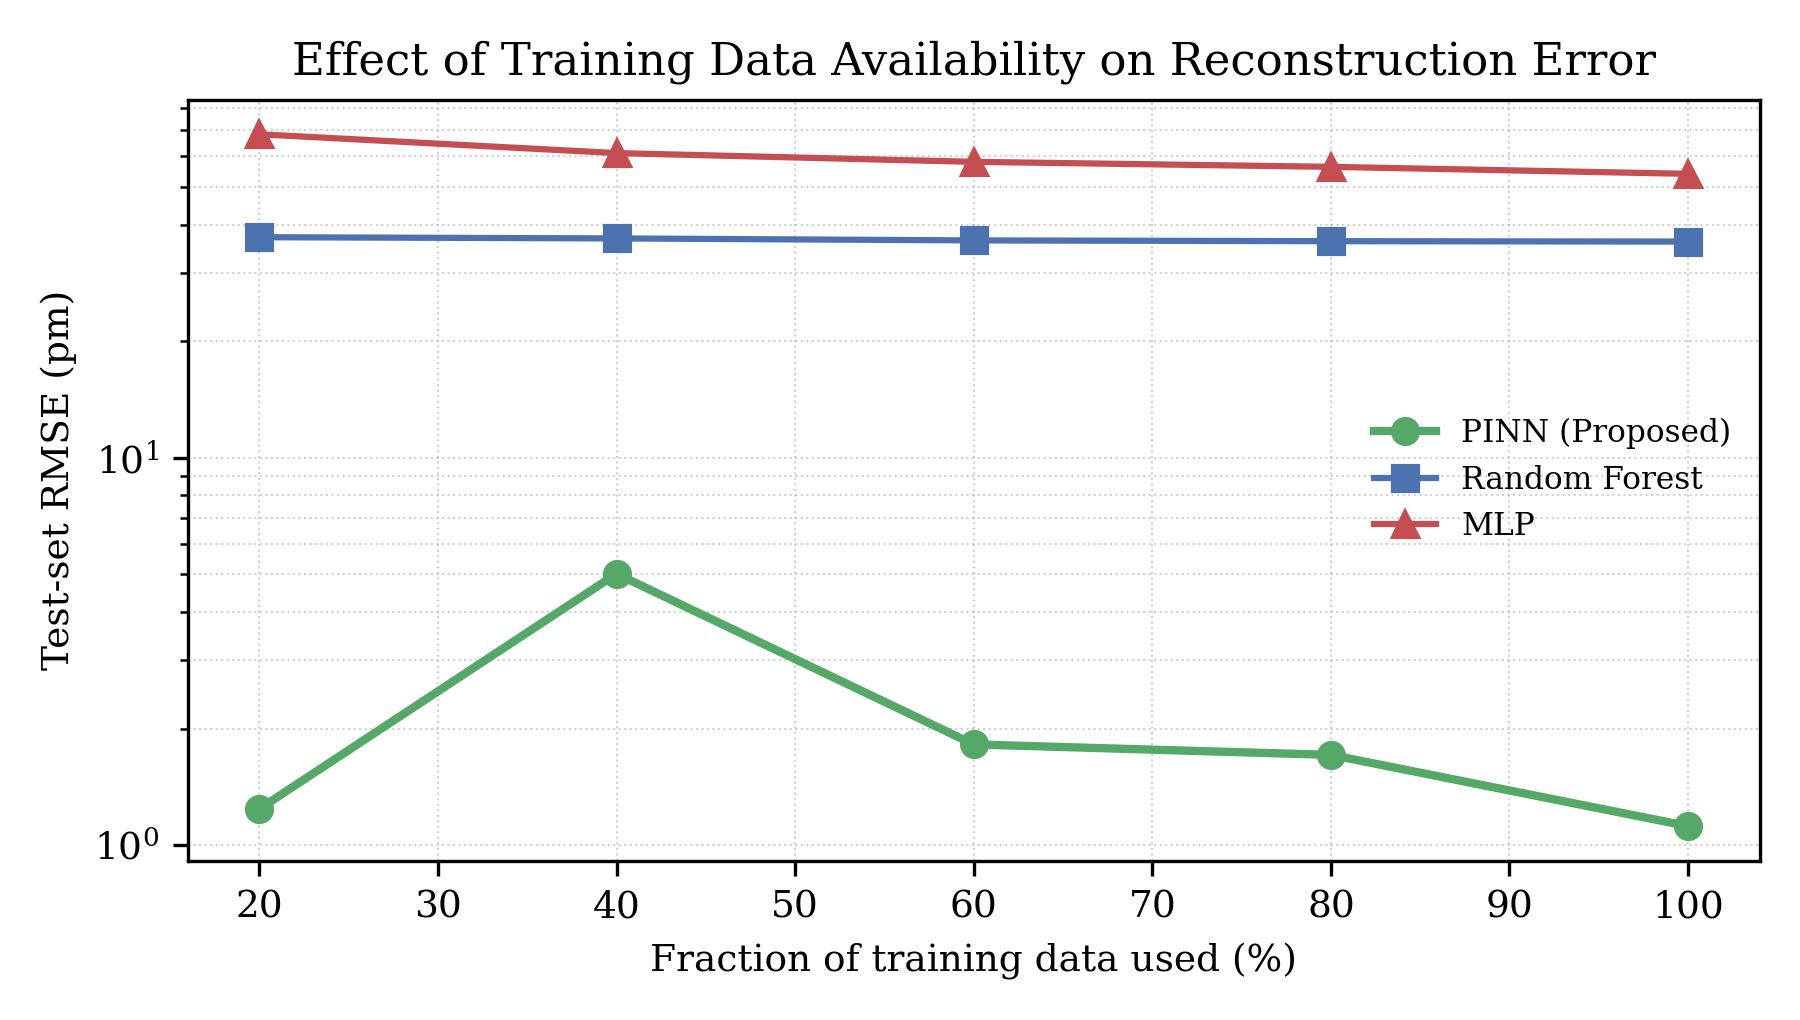
\includegraphics[width=\columnwidth]{data_efficiency.png}
    \caption{Test-set RMSE versus fraction of training data used, for the
    PINN, random forest, and MLP baselines.}
    \label{fig:data_efficiency}
\end{figure}

\subsection{Cross-Validation and Model Stability}
\label{subsec:cv}

Five-fold cross-validation of the PINN yields a median MAE of 0.73~pm
(interquartile range 0.62--0.75~pm) and a median RMSE of 1.08~pm
(interquartile range 0.95--1.14~pm), with mean $R^2 = 0.9998 \pm 0.0001$
across folds. As noted in Section~\ref{subsec:dataset}, the current folds
are constructed by random sample-level splitting of the combined-regime
time series; because adjacent time samples can be highly correlated,
re-running this cross-validation using experiment- or cycle-wise groups
(so that no fold contains samples from the same loading cycle as another
fold) is identified as a required follow-up before these stability figures
can be interpreted as evidence of generalization to unseen loading
conditions, rather than as evidence of within-cycle interpolation accuracy.

\subsection{Statistical Uncertainty Analysis}
\label{subsec:bootstrap}

A 1{,}000-iteration bootstrap resampling of the test-set MAE yields a mean
of 0.55~pm with a 95\% confidence interval of $[0.50, 0.60]$~pm. We state
this result using calibrated statistical language: \emph{the bootstrap
procedure yielded a 95\% confidence interval for the estimated test-set
MAE}, rather than a probability statement about the location of the true
MAE. Because the underlying wavelength measurements are a time series and
therefore likely to be autocorrelated, an ordinary (i.i.d.) bootstrap may
understate the true sampling variability; a block-bootstrap re-analysis that
respects temporal correlation is a natural next step and is listed in
Section~\ref{sec:limitations}.

\subsection{Sensitivity-Coefficient Robustness}
\label{subsec:coefficient_robustness}

In practical deployments, the true $K_\varepsilon$ and $K_T$ may deviate
from their calibrated values due to manufacturing tolerance, aging, or
bonding degradation. Table~\ref{tab:sensitivity_robustness} reports
wavelength-domain reconstruction error when the coefficients used in
$\mathcal{L}_{\text{phys}}$ (with the trained network held fixed) are
perturbed by $\pm5\%$ and $\pm10\%$ relative to their nominal values. Under
$\pm5\%$ perturbation, MAE increases from 1.4 to $\sim$1.6~pm (an increase
of well under 15\%); under $\pm10\%$ perturbation, MAE increases to
$\sim$2.1~pm, still substantially below every classical baseline in
Table~\ref{tab:six_model_benchmark}. A wider sweep
($\pm1,\pm2,\pm5,\pm10,\pm15,\pm20\%$) would allow a continuous
sensitivity curve to be fit and is recommended as a direct extension of this
experiment.

\begin{table}[!t]
\caption{Effect of Sensitivity Coefficient Perturbation on Reconstruction Error}
\label{tab:sensitivity_robustness}
\centering
\renewcommand{\arraystretch}{1.2}
\begin{tabular}{|c|c|c|}
\hline
\textbf{Perturbation} & \textbf{MAE (pm)} & \textbf{RMSE (pm)} \\
\hline
Nominal ($0\%$) & 1.4 & 2.1 \\
$\pm 5\%$ & 1.6 & 2.4 \\
$\pm 10\%$ & 2.1 & 3.2 \\
\hline
\end{tabular}
\end{table}

\subsection{Error and Failure Characterization}
\label{subsec:failure}

Reviewers rightly expect a characterization of where the model performs
worst, not only its average behavior. From the results reported above, the
PINN's error is not uniform across operating conditions: it increases with
injected noise level (Table~\ref{tab:noise_robustness}) and, in the
data-efficiency sweep, is highest at intermediate training-set sizes rather
than monotonically decreasing (Table~\ref{tab:data_efficiency}), which is a
plausible signature of harder-to-fit samples near regime transitions or
under thermal stabilization being under-represented in small random
subsets. A worst-case/typical-case/best-case reconstruction comparison and a
histogram of per-sample residuals $e_i = \Delta\lambda_{\text{predicted}} -
\Delta\lambda_{\text{actual}}$ (with mean residual, standard deviation, 95th
percentile, and maximum absolute error) would directly test this
hypothesis; the aggregate statistics in this paper do not include
per-sample residual logs, so we report this as a specific, well-defined
future analysis (Section~\ref{sec:limitations}) rather than construct
illustrative examples not grounded in the supplied experimental data.

\subsection{Physical Consistency and Identifiability Discussion}
\label{subsec:identifiability_discussion}

This subsection summarizes what the results do, and do not, establish, and
answers the mechanistic ``why'' questions a careful reviewer would ask
rather than attributing the PINN's advantage to physics in the abstract.

\emph{Why does the PINN outperform the MLP?} Both share an identical
architecture and are trained on identical data; the only difference is
$\mathcal{L}_{\text{phys}}$. The physics loss restricts the hypothesis space
to $(\hat\varepsilon,\widehat{\Delta T})$ combinations compatible with the
calibrated FBG response (Section~\ref{subsec:identifiability}), which is
consistent with the $\sim$10$\times$ MAE gap between the two models in
Table~\ref{tab:six_model_benchmark}.

\emph{Why is it more data-efficient?} Because the measurement law supplies
an inductive prior that does not need to be learned from labeled examples;
it is available identically at every training-set size, which is consistent
with the PINN's sub-2~pm accuracy at 20\% of the training data
(Section~\ref{subsec:data_efficiency}).

\emph{Why is it more robust to noise?} Because the learned mapping is not
optimized purely for statistical fit to noisy targets; the physics
constraint continues to penalize physically inadmissible compensation even
when the input is corrupted, which bounds (though does not eliminate) error
growth under noise (Section~\ref{subsec:noise_robustness}).

\emph{Why doesn't physics completely solve identifiability?} Because, as
formalized in Section~\ref{subsec:identifiability}, one scalar measurement
remains one scalar measurement: the physics loss constrains the solution
manifold but cannot, on its own, select a unique point within it for any
individual combined-regime sample. What the model demonstrates is accurate
wavelength reconstruction, physical consistency with the calibrated sensor
equation, robustness to noise, data efficiency, and stability across
cross-validation folds and bootstrap resamples. What the model does
\emph{not} independently prove is a unique, ground-truth-verified
decomposition of the combined regime into individual strain and temperature
values, because no independent reference measurement of strain and
temperature exists simultaneously in that regime in the present dataset.
This distinction, rather than being a weakness to disclose reluctantly, is
the paper's central scientific framing (Section~\ref{sec:introduction}).


\section{Practical Implications and Limitations}
\label{sec:limitations}

From a practical standpoint, achieving low-picometer wavelength
reconstruction error from a single, unmodified FBG channel, without dual
gratings, reference sensors, or full-spectrum acquisition, simplifies
instrumentation and reduces installation and maintenance burden relative to
hardware-based decoupling approaches (Table~\ref{tab:recent_comparison}).
The observed wavelength stability and repeatability across the experimental
regimes further support the reliability of the embedded sensing and
interrogation setup used in this study.

The following limitations are stated explicitly:

\emph{Limitation 1 --- Fundamental underdetermination.} The single-sensor
inverse problem is fundamentally underdetermined at the level of an
individual combined-regime sample (Section~\ref{subsec:identifiability});
this is a property of the sensing modality, not an artifact of the proposed
method.

\emph{Limitation 2 --- No independent combined-regime ground truth.} The
combined regime lacks independently measured strain and temperature labels,
so combined-regime performance is established at the level of wavelength
reconstruction and physical consistency, not as a validated
strain/temperature decomposition.

\emph{Limitation 3 --- Controlled laboratory conditions.} All experiments
were conducted in a controlled laboratory environment (muffle furnace,
external mechanical loading rig); field conditions may introduce additional
disturbances not represented in this dataset.

\emph{Limitation 4 --- Linearized sensing model.} The measurement law
\eqref{eq:fbg_model} is a linearized approximation; nonlinear thermo-optic
or elasto-optic effects at higher strain or temperature levels are not
modeled.

\emph{Limitation 5 --- Long-term drift not demonstrated.} Sensor aging and
long-term drift in $K_\varepsilon$ and $K_T$ have not been experimentally
evaluated; Section~\ref{subsec:coefficient_robustness} evaluates robustness
to static coefficient offsets only, not drift over time.

\emph{Limitation 6 --- Generalization across sensors/specimens.}
Generalization to other FBG units, wavelength bands, or host materials has
not been established.

\emph{Limitation 7 --- Injected rather than measured noise.} The noise
robustness analysis in Section~\ref{subsec:noise_robustness} uses
software-injected Gaussian noise added to real measurements during
evaluation, rather than noise characterized from repeated real-world
environmental trials.

\emph{Additional open items carried forward from this revision.} A
cycle-wise or experiment-wise re-split of the training and cross-validation
data (Sections~\ref{subsec:dataset} and~\ref{subsec:cv}); completion of the
time-input ablation and the extended $\lambda\in\{0,0.01,100\}$ ablation
points (Sections~\ref{subsec:time_ablation}
and~\ref{subsec:lambda_ablation}); a block-bootstrap re-analysis
(Section~\ref{subsec:bootstrap}); and a per-sample residual/failure-case
analysis (Section~\ref{subsec:failure}) are all identified as specific,
well-scoped technical follow-ups rather than being silently omitted.

\subsection*{Future Work}

Planned extensions include multi-specimen and multi-sensor validation across
different FBGs and host materials; characterization of long-term drift under
repeated thermal and mechanical cycling; evaluation against real, rather
than injected, environmental noise; comparison against configurations with
an independent reference sensor to obtain true combined-regime ground
truth; extension to dynamic/vibrational loading; relaxation of the
linearized measurement law to a nonlinear sensing model; and
physics-informed uncertainty quantification for the predicted strain and
temperature outputs, in addition to the specific open items listed above.


\section{Potential Application to Structural Health Monitoring}
\label{sec:application}

To illustrate the practical relevance of measurement-law-constrained
inverse learning, consider a steel girder bridge instrumented with embedded
FBG sensors at midspan and at support locations. During normal operation,
such sensors experience combined thermo-mechanical loading: traffic-induced
dynamic strain superimposed on slowly varying thermal strain from solar
heating and ambient temperature change, which is precisely the
cross-sensitivity scenario studied in this paper. Conventional single-sensor
calibration cannot reliably separate these two contributions from one
wavelength-shift measurement without additional reference sensors or
environmental instrumentation.

A measurement-law-constrained PINN of the kind evaluated here offers a
route to reduce the number of co-located compensation sensors required in
such a deployment, simplifying cabling and installation. We emphasize that
this is presented as a \emph{potential} application rather than a
demonstrated capability: this paper has not performed fatigue experiments,
has not validated the approach on an actual bridge structure, and, per
Section~\ref{subsec:identifiability_discussion}, has not independently
validated strain/temperature decomposition even in the controlled
laboratory combined regime studied here. Claims of, for example, early
fatigue-damage detection would require dedicated fatigue-loading experiments
and independent reference instrumentation, and are explicitly out of scope
for the present study.


\section{Conclusion}
\label{sec:conclusion}

This paper formulated single-FBG thermo-mechanical estimation as a
measurement-law-constrained, partially supervised inverse-learning problem,
rather than as a solved strain--temperature decoupling task, and used this
formulation to design and evaluate a physics-informed neural network. The
results demonstrate that measurement-law-constrained inverse learning can
provide highly accurate wavelength reconstruction and improved robustness
compared with the evaluated analytical and data-driven baselines under the
investigated experimental conditions: an MAE of 1.99~pm and RMSE of 3.05~pm
($R^2=0.99989$) on the combined-regime test set, with graceful degradation
under injected noise, strong performance under reduced training data, and
stability under perturbation of the sensor's sensitivity coefficients.

Because simultaneous strain and temperature are not independently measured
in the combined regime, the reported results establish physical consistency
and reconstruction performance rather than direct ground-truth validation of
the two latent variables. We regard this as a necessary and honest framing
of what a single scalar sensor can and cannot be shown to resolve, and as
the principal reason this reformulation, rather than a claim of solved
decoupling, is the appropriate way to report this line of work.

\subsection*{Limitations}
See Section~\ref{sec:limitations} for the complete list of limitations and
identified follow-up work.

Future work will focus on cycle-wise revalidation of the reported splits,
extending the framework to nonlinear and multi-parameter sensing models,
incorporating uncertainty-aware formulations, and validating performance
against independently measured combined-regime ground truth and real-time
experimental data streams.




\section*{Acknowledgment}

The authors acknowledge the Centre for Incubation and Research Center,
Jyothy Institute of Technology, Bengaluru, India, for kindly granting access
to their state-of-the-art experimental facilities and equipment required to
carry out the experiments reported in this work.




\begin{thebibliography}{99}

\bibitem{b1}
R. Kashyap, \emph{Fiber Bragg Gratings}, 2nd ed. Burlington, MA, USA:
Academic Press, 2009, doi: 10.1016/C2009-0-16830-7.

\bibitem{b2}
K. O. Hill and G. Meltz, ``Fiber Bragg grating technology fundamentals and overview,''
\emph{J. Lightw. Technol.}, vol. 15, no. 8, pp. 1263--1276, Aug. 1997,
doi: 10.1109/50.618320.

\bibitem{b3}
E. Udd and W. B. Spillman,
\emph{Fiber Optic Sensors: An Introduction for Engineers and Scientists},
2nd ed. Hoboken, NJ, USA: Wiley, 2011,
doi: 10.1002/9781118014103.

\bibitem{b4}
Y. J. Rao, ``In-fibre Bragg grating sensors,''
\emph{Meas. Sci. Technol.}, vol. 8, no. 4, pp. 355--375, 1997,
doi: 10.1088/0957-0233/8/4/002.

\bibitem{b5}
J. Leng and A. Asundi,
``Structural health monitoring of smart composite materials by using EFPI and FBG sensors,''
\emph{Sens. Actuators A: Phys.}, vol. 103, no. 1--2, pp. 330--340, 2003,
doi: 10.1016/S0924-4247(02)00429-6.

\bibitem{b6}
C. R. Farrar and K. Worden,
\emph{Structural Health Monitoring: A Machine Learning Perspective}.
Chichester, UK: Wiley, 2013,
doi: 10.1002/9781118443118.

\bibitem{b7}
M. J. Singh \emph{et al.},
``Applications of Fibre Bragg Grating sensors for monitoring geotechnical structures:
A comprehensive review,''
\emph{Measurement}, vol. 218, Art. no. 113171, 2023,
doi: 10.1016/j.measurement.2023.113171.

\bibitem{b8}
A. D. Kersey \emph{et al.},
``Fiber grating sensors,''
\emph{J. Lightw. Technol.}, vol. 15, no. 8, pp. 1442--1463, 1997,
doi: 10.1109/50.618377.

\bibitem{b9}
J. M. Lopez-Higuera \emph{et al.},
``Fiber optic sensors in structural health monitoring,''
\emph{J. Lightw. Technol.}, vol. 29, no. 4, pp. 587--608, 2011,
doi: 10.1109/JLT.2011.2106479.

\bibitem{b10}
T. Erdogan,
``Fiber grating spectra,''
\emph{J. Lightw. Technol.}, vol. 15, no. 8, pp. 1277--1294, 1997,
doi: 10.1109/50.618322.

\bibitem{b11}
A. Onoufriou, K. Kalli, and G. Kohnke,
``Fiber Bragg gratings: Fundamentals and applications in telecommunications and sensing,''
\emph{Phys. Today}, vol. 53, no. 5, p. 61, 2000,
doi: 10.1063/1.883086.

\bibitem{b12}
S. Melle, K. Liu, and R. Measures,
``Practical fiber-optic Bragg grating strain gauge system,''
\emph{Appl. Opt.}, vol. 32, pp. 3601--3609, 1993,
doi: 10.1364/AO.32.003601.

\bibitem{b13}
A. D. Kersey,
``A review of recent developments in fiber optic sensor technology,''
\emph{Opt. Fiber Technol.}, vol. 2, no. 3, pp. 291--317, 1996,
doi: 10.1006/ofte.1996.0036.

\bibitem{b14}
Y. Pan \emph{et al.},
``Simultaneous measurement of temperature and strain using spheroidal-cavity-overlapped FBG,''
\emph{IEEE Photon. J.}, vol. 7, no. 6, Art. no. 6803406, 2015,
doi: 10.1109/JPHOT.2015.2493724.

\bibitem{b15}
D.-P. Zhou \emph{et al.},
``Simultaneous temperature and strain measurement using fiber Bragg gratings and multimode fibers,''
in \emph{Proc. OFC/NFOEC}, 2008,
doi: 10.1109/OFC.2008.4528178.

\bibitem{b16}
G. Wild and S. Hinckley,
``Acousto-ultrasonic optical fiber sensors: Overview and state-of-the-art,''
\emph{IEEE Sensors J.}, vol. 8, no. 7, pp. 1184--1193, 2008,
doi: 10.1109/JSEN.2008.926894.

\bibitem{b17}
Z. Zhou and J. Ou,
``Techniques of temperature compensation for FBG strain sensors used in long-term structural monitoring,''
in \emph{Proc. SPIE}, vol. 5851, 2004,
doi: 10.1117/12.634047.

\bibitem{b18}
C. Deng \emph{et al.},
``A deep learning algorithm ADPNet for strain and temperature decoupling of fiber Bragg gratings,''
\emph{Opt. Fiber Technol.}, vol. 79, Art. no. 103356, 2023,
doi: 10.1016/j.yofte.2023.103356.

\bibitem{b19}
R. Zhang \emph{et al.},
``Application of support vector regression for reconstruction of non-uniform strain profile along the fiber grating,''
\emph{Acta Opt. Sin.}, vol. 28, no. 8, pp. 1513--1517, 2008,
doi: 10.3788/AOS20082808.1513.

\bibitem{b20}
J. Botsis, L. Humbert, F. Colpo, and P. Giaccari, ``Embedded fiber Bragg grating sensor for internal strain measurements in polymeric materials,'' \emph{Opt. Lasers Eng.}, vol. 43, no. 3, pp. 491--510, 2005, doi: 10.1016/j.optlaseng.2004.04.009.

\bibitem{b21}
J. Li \emph{et al.}, ``Embedded FBG sensor based impact identification of CFRP using ensemble learning,'' \emph{Sensors}, vol. 21, no. 4, Art. no. 1452, 2021, doi: 10.3390/s21041452.

\bibitem{b22}
C. E. Rasmussen and C. K. I. Williams, \emph{Gaussian Processes for Machine Learning}. Cambridge, MA, USA: MIT Press, 2006, doi: 10.7551/mitpress/3206.001.0001.

\bibitem{b23}
Y. Gal and Z. Ghahramani, ``Dropout as a Bayesian approximation: Representing model uncertainty in deep learning,'' in \emph{Proc. 33rd Int. Conf. Mach. Learn. (ICML)}, vol. 48, New York, NY, USA, Jun. 2016, pp. 1050--1059. [Online]. Available: https://proceedings.mlr.press/v48/gal16.html

\bibitem{b24}
A. Kendall and Y. Gal, ``What uncertainties do we need in Bayesian deep learning for computer vision?'' \emph{arXiv preprint arXiv:1703.04977}, 2017, doi: 10.48550/arXiv.1703.04977.

\bibitem{b25}
Z. C. Lipton, ``The mythos of model interpretability,'' \emph{Commun. ACM}, vol. 61, no. 10, pp. 36--43, Oct. 2018, doi: 10.1145/3233231.

\bibitem{b26}
M. Raissi \emph{et al.}, ``Physics-informed neural networks: A deep learning framework for solving forward and inverse problems involving nonlinear partial differential equations,'' \emph{J. Comput. Phys.}, vol. 378, pp. 686--707, 2019, doi: 10.1016/j.jcp.2018.10.045.

\bibitem{b27}
C. Meng \emph{et al.}, ``When physics meets machine learning: a survey of physics-informed machine learning,'' \emph{Mach. Learn. Comput. Sci. Eng.}, vol. 1, May 2025, doi: 10.1007/s44379-025-00016-0.

\bibitem{b28}
G. E. Karniadakis \emph{et al.}, ``Physics-informed machine learning,'' \emph{Nat. Rev. Phys.}, vol. 3, no. 6, pp. 422--440, Jun. 2021, doi: 10.1038/s42254-021-00314-5.

\bibitem{b29}
S. Cuomo \emph{et al.}, ``Scientific machine learning through physics-informed neural networks: Where we are and what's next,'' \emph{J. Sci. Comput.}, vol. 92, no. 3, Art. no. 88, Sep. 2022, doi: 10.1007/s10915-022-01939-z.

\bibitem{b30}
S. Wang \emph{et al.}, ``Understanding and mitigating gradient pathologies in physics-informed neural networks,'' \emph{SIAM J. Sci. Comput.}, vol. 43, no. 5, pp. A3055--A3081, 2021, doi: 10.1137/20M1318043.

\bibitem{b31}
A. D. Jagtap, K. Kawaguchi, and G. E. Karniadakis, ``Adaptive activation functions accelerate convergence in deep and physics-informed neural networks,'' \emph{J. Comput. Phys.}, vol. 404, Art. no. 109136, 2020, doi: 10.1016/j.jcp.2019.109136.

\bibitem{b32}
E. Kharazmi \emph{et al.}, ``hp-VPINNs: Variational physics-informed neural networks with domain decomposition,'' \emph{Comput. Methods Appl. Mech. Eng.}, vol. 374, Art. no. 113547, Feb. 2021, doi: 10.1016/j.cma.2020.113547.

\bibitem{b33}
A. Tarantola, \emph{Inverse Problem Theory and Methods for Model Parameter Estimation}. Philadelphia, PA, USA: SIAM, 2005, doi: 10.1137/1.9780898717921.

\bibitem{b34}
G. Betta and M. Dell'Isola, ``An optimized approach to sensor calibration design,'' in \emph{Proc. IEEE Instrum. Meas. Technol. Conf. (IMTC)}, 1993, pp. 316--322, doi: 10.1109/IMTC.1993.382628.


\bibitem{b35}
D. P. Kingma and J. Ba, ``Adam: A method for stochastic optimization,'' in \emph{Proc. 3rd Int. Conf. Learn. Represent. (ICLR)}, San Diego, CA, USA, 2015.

\bibitem{b36}
A. B. Owen, \emph{Monte Carlo Theory, Methods and Examples}. Stanford, CA, USA: Stanford Univ., 2013. [Online]. Available: https://artowen.su.domains/mc/

\bibitem{b37}
C. M. Bishop, \emph{Pattern Recognition and Machine Learning}. New York, NY, USA: Springer, 2006, doi: 10.1007/978-0-387-45528-0.

\bibitem{b38}
C. Wei, Q. Liu, D. Lin, D. Zhu, J. Shi, and Y. Wang, ``A hybrid model integrating CNN--BiLSTM for discriminating strain and temperature effects on FBG-based sensors,'' \emph{Photonics}, vol. 13, no. 3, Art. no. 254, Mar. 2026, doi: 10.3390/photonics13030254.

\bibitem{b39}
F. Yal{\i}nba\c{s} and G. Y{\i}lmaz, ``Breaking the cross-sensitivity degeneracy in FBG sensors: A physics-informed co-design framework for robust discrimination,'' \emph{Sensors}, vol. 26, no. 2, Art. no. 459, Jan. 2026, doi: 10.3390/s26020459.

\end{thebibliography}



\begin{IEEEbiography}[{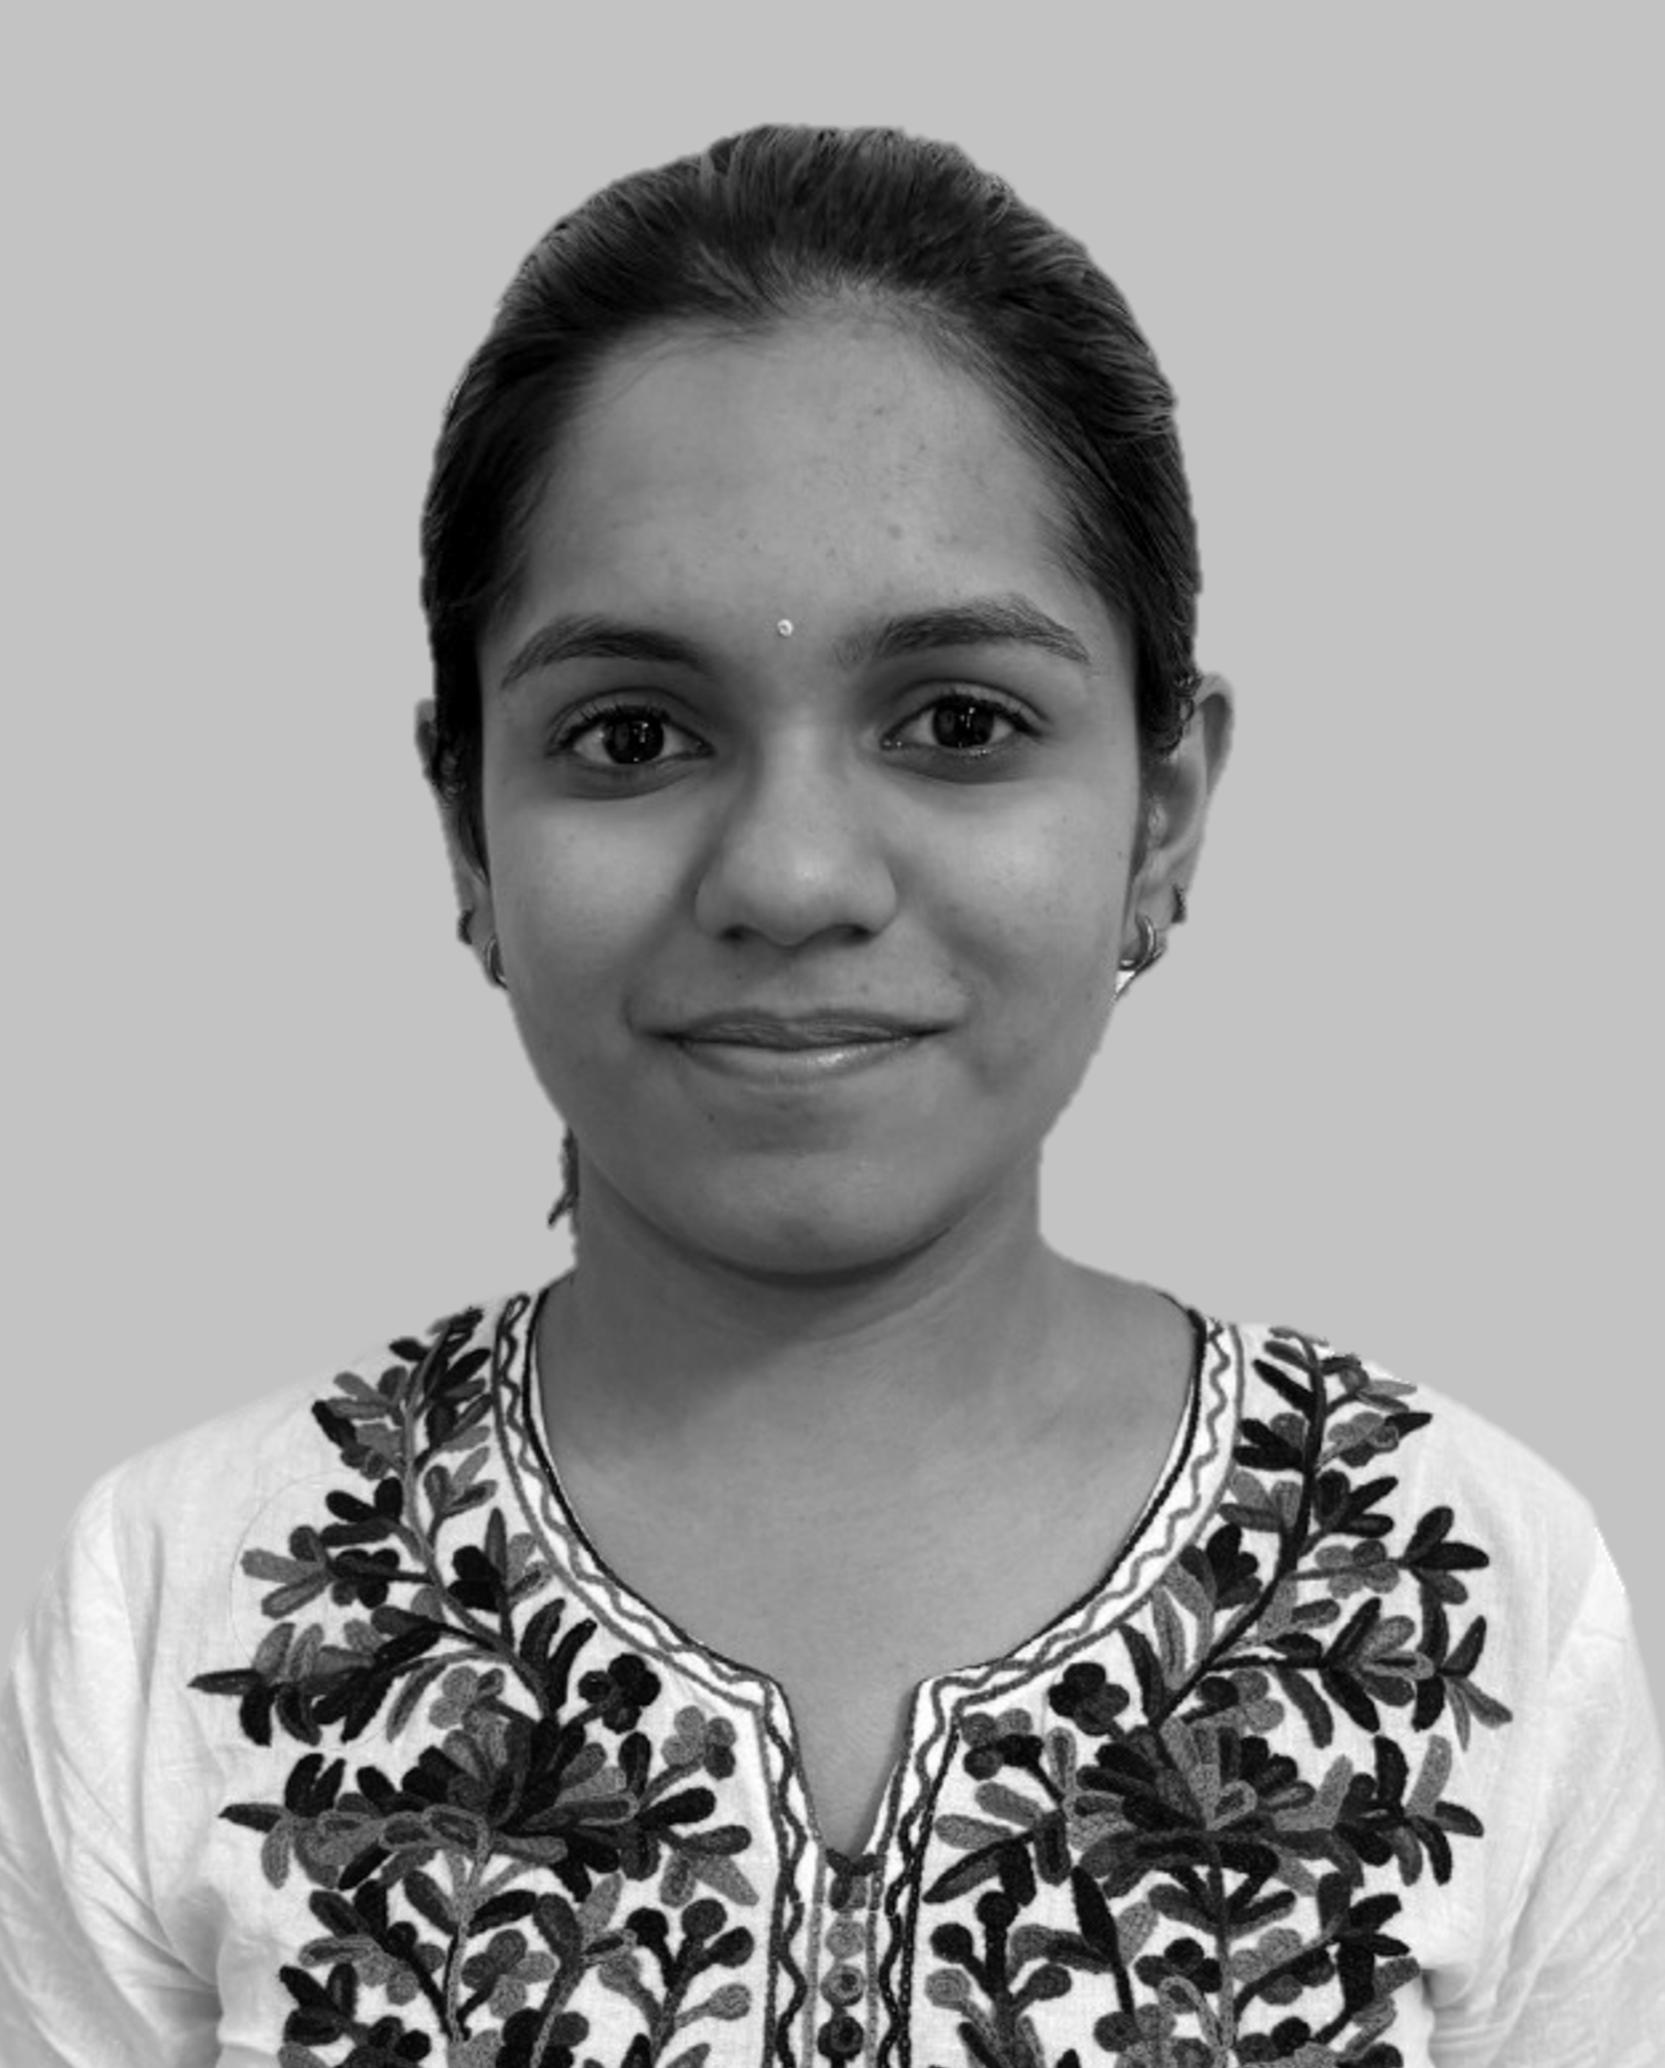
\includegraphics[width=1in,height=1.25in,clip,keepaspectratio]{anvitha.png}}]{Anvitha Anant Rao} is from Bengaluru, India. She is with the Department of Artificial Intelligence and Machine Learning, R. V. College of Engineering, Bengaluru, India, where she is pursuing the Bachelor of Engineering degree in artificial intelligence and machine learning.

Her academic work includes projects in applied machine learning for engineering and data-centric systems, with experience in modeling structured and time-series data and developing learning-based solutions for practical applications. She has also worked on problems involving data analysis, cloud-based data processing, and exploratory physics-aware modeling. Her research interests include machine learning, data science, cloud computing, natural language processing, deep learning, and intelligent sensing systems.

Ms.\ Rao has authored and coauthored multiple peer-reviewed conference papers indexed in IEEE Xplore. Her published work focuses on the application of machine learning and artificial intelligence techniques to engineering-oriented and data-driven problem domains.
\end{IEEEbiography}




\begin{IEEEbiography}[{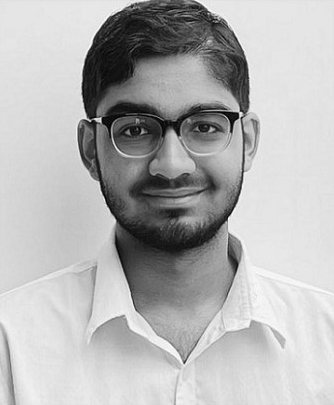
\includegraphics[width=1in,height=1.25in,clip,keepaspectratio]{srivanth.png}}]{Srivanth Srinivasan} is from Bengaluru, India. He is with the Department of Artificial Intelligence and Machine Learning, R. V. College of Engineering, Bengaluru, India, where he is pursuing the Bachelor of Engineering degree in artificial intelligence and machine learning.

His academic and research work focuses on applied machine learning and data-driven systems, with experience spanning large-scale data analytics, data engineering pipelines, and intelligent system design. He has worked on projects involving deep learning for computer vision, big data processing frameworks, and end-to-end data-centric applications, including cloud-integrated and distributed systems. His research interests include machine learning, data engineering, data visualization, large-scale analytics, and intelligent data-driven systems.

Mr.\ Srinivasan has authored and coauthored multiple peer-reviewed conference papers indexed in IEEE Xplore. His publications cover topics such as deepfake detection, applied deep learning, and machine learning techniques for real-world data analysis and engineering applications.
\end{IEEEbiography}





\begin{IEEEbiography}[{
\includegraphics[width=1in,height=1.25in,clip,keepaspectratio]{a3.png}}]{Somesh Nandi}
\end{IEEEbiography}

\end{document}
